\documentclass[a4paper, oneside, openany, dvipdfmx]{suribt}% 本文が * ページ以下のときに (掲示に注意)
\usepackage{graphicx}
\usepackage{newtxtext,newtxmath}
\usepackage{amsmath}
\usepackage{mathtools}
\usepackage{slashbox}
\usepackage[unicode, ipaex]{pxchfon}
\usepackage{here}
\usepackage[hang,small,bf]{caption}
\usepackage[subrefformat=parens]{subcaption}
\captionsetup{compatibility=false}
\title{事前学習がVision Transformerに与える影響}
%\titlewidth{}% タイトル幅 (指定するときは単位つきで)
\author{桝田 修慎}
\eauthor{Masachika Masuda}% Copyright 表示で使われる
\studentid{18A1066}
\supervisor{山口裕 助教}% 1 つ引数をとる (役職まで含めて書く)
%\supervisor{指導教員名 役職 \and 指導教員名 役職}% 複数教員の場合,\and でつなげる
\handin{2022}{2}% 提出月. 2 つ (年, 月) 引数をとる
\keywords{Vision Transformer} % 概要の下に表示される

%・データ構成とはなにか、>>> 2章ではどんなことをして、3章ではどんなことをするのか…
%・実験結果の図が多い、付録に入れるべきか >>> 卒論であればメインに入れ込んで良い
%・データ拡張の図は理論のところに入れるべきか、手順のところにいれるべきか >>> 上に同じ
%・サブセクションまで目次に表示させるべきか >>> どちらでも良い
%・図は基本的に自作 >>> 自作、元論文とほとんど同じ場合は引用する
%・図のグリッドは必要か >>> どちらでも良い

\newcommand{\fref}[1]{図\ref{#1}}
\newcommand{\tref}[1]{表\ref{#1}}
\newcommand{\eref}[1]{式\eqref{#1}}

\begin{document}
\maketitle%%%%%%%%%%%%%%%%%%% タイトル %%%%

\frontmatter% ここから前文
\begin{abstract}%%%%%%%%%%%%% 概要 %%%%%%%%
画像認識分野では,畳み込み層を重ねることで良い認識結果をもたらしたVGGをはじめ,残差機構を取り入れ,更に層を深くすることを可能にしたResNetがState-of-the-artを達成し,デファクトスタンダードとなっていた.
しかし,今回のテーマであるVision Transformerは畳み込み層を使っておらず,Attention層を用いて代用している.
また,Vision Transformerでの大規模なデータセットを用いた事前学習は,認識結果に影響し,ImageNet ReaL,CIFAR-100,VTABなどの画像認識のベンチマークでState-of-the-artを達成し,更新した.
そこで本研究では,Vision Transformerを用いて,各自で用意したデータセットに対して事前学習をおこなった場合とそうでない場合,事前学習のデータセット規模を変えた場合で認識結果を向上させることができるのか検証した.

\end{abstract}

\setcounter{tocdepth}{2}
\tableofcontents%%%%%%%%%%%%% 目次 %%%%%%%%

\mainmatter% ここから本文 %%% 本文 %%%%%%%%
\chapter{序論}
\section{背景}
近年,画像認識分野では,機械翻訳で脚光を浴びることになったTransformer\cite{vaswani2017attention}をコンピュータビジョンに適応させたVision Transformer(以下ViTと称する)が登場した\cite{dosovitskiy2021image}.
ViTは,層を深くし畳み込みを行う畳み込みニューラルネットワーク(以下CNNと称する)とは違い,畳み込み演算をAttention機構を用いて代用しており,特に大規模なデータで事前学習を行なったときの,小・中規模の画像認識ベンチマーク(ImageNet ReaL,CIFAR-100,VTAB,etc.)では,
過去のState-of-the-artのCNNモデルと比べて少ない計算リソースで訓練することができ、更に素晴らしい結果も出している.

本研究では,Vision Transformerが提案された論文
「An Image is Worth 16x16 Words: Transformers for Image Recognition at Scale」を参考にし,事前学習やデータ拡張の有無が,学習及び推論に与える影響を検証した.
\section{本研究の目的}
本研究の目的を以下に示す.
\begin{enumerate}
  \item 一定の条件下での振る舞いを従来のモデル(VGG,ResNet)と比較し,ViTの優れている点・そうではない点を明らかにする.
  \item 事前学習やデータ拡張が各モデルに及ぼす影響を調べる.
\end{enumerate}

\section{深層学習}
深層学習とは,脳の神経回路を模したニューラルネットワークをより深くしたものを指す.現在では画像のみならず,音声,自然言語など多くの分野に対して優れた性能を発揮している.
\subsection{畳み込みニューラルネットワーク}
畳み込みニューラルネットワーク(CNN)は,入力した画像に対してカーネルを移動させながらスカラ積を求めていく畳み込み層を複数重ねているネットワークのことである.
カーネルは画像全体に同じものを適用するため,CNNは移動させたカーネルと画像のスカラ積による局所性と,画像全体に渡る同一カーネルの重みの使用による移動不変性を持つ.
%移動不変性:局所的なパターンが画像内の物体位置にかかわらず、出力に対して効果的であること.局所性:近傍における局所的な演算処理
\subsection{VGG}
VGGはCNNの一種で,3x3という小さいカーネルを用いており,2014年当時では珍しい16層及び19層の深いネットワークである\cite{simonyan2015deep}.
畳み込みとプーリング,線形層のシンプルなアーキテクチャであるにも関わらず,2014年のImageNetチャレンジのローカリゼーション・クラシフィケーションタスクで1位と2位を収めている.

\subsection{ResNet}
一般的に,CNNでは層を重ねることで,より高次元な特徴を抽出することができるが,層が深くなるにつれて勾配が発散・消失するという問題があった.
しかし,ResNetは,畳み込み層を重ねるだけではなく,浅い層の出力を次の層の入力とする残差機構(スキップ接続)を取り入れることで,より畳み込み層を多く積み重ねながらも,SoTAを達成した\cite{he2015deep}.
ResNetのブロックの一部を\fref{fig:res_arch}に示す.入力を$x$とし,2層のweight layer(畳み込み層)を$f(x)$とする.入力$x$はweight layerと活性化関数ReLUを経由し,$f(x)$として出力される.
そしてスキップ接続の$x$を加算し,最終的な出力は$f(x)+x$である.
\begin{figure}[H]
  \centering
  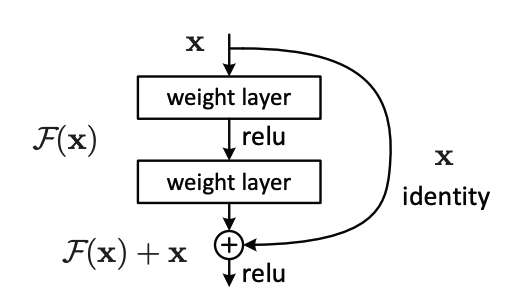
\includegraphics[width=0.9\linewidth]{figs/resnet.png}
  \caption{ResNetのアーキテクチャ(一部)\cite{he2015deep}}
  \label{fig:res_arch}
\end{figure}
\subsection{Transformer}
\label{sec:attention}
Transformerは,それまで機械翻訳モデルで多く使われてきた畳み込みニューラルネットワーク・再帰ニューラルネットワークのような複雑なアーキテクチャを持つネットワークとは違い
Attention機構のみを用いて構成されているエンコーダ・デコーダモデルである\cite{vaswani2017attention}.
Transformerのアーキテクチャを\fref{fig:tr_arch}に示す.

Attention機構から求まるAttentionは,文章中の単語間の関連度のようなもので,ある単語を理解するのに,どの単語に注目すれば良いかを定量的に示すことができる.
また,一つの文章中の単語のみで求めるAttentionはSelf-Attentionと呼び,以降,AttentionはSelf-Attentionを指す.
%また,今回扱う一つの文章中の単語のみで求めるAttentionはSelf-Attentionと呼ばれる.以降,AttentionはSelf-Attentionを示す.

Attentionを求める例として,「I like an apple, it is delicious.」という文章を考える.
初めに,文字列「I like an apple, it is delicious.」を入力とする.入力は単語ごとにベクトルに埋め込まれ$x_{1},...,x_{7}$と表し,次元は$d_{model}$で,論文\cite{vaswani2017attention}より512である.
また,今回は簡単のためにカンマとピリオドは省略している.
$x_{1},...,x_{7}$はそれぞれ訓練過程で学習された重み行列$W_{Q},W_{K},W_{V}$と掛け合わせ,それぞれ$q_{1},...,q_{7}, k_{1},...,k_{7}, v_{1},...,v_{7}$とする.
また,$d_{q}=d_{k}=d_{v}=64,\ W_{Q}\in \mathbb{R}^{d_{model}\times d_{k}}, W_{K}\in \mathbb{R}^{d_{model}\times d_{k}},  W_{V}\in \mathbb{R}^{d_{model}\times d_{v}}$である.
今回は,「it」に対してのAttentionを求める.「it」は先頭から5文字目なので,生成されたベクトル$q_{5}, k_{5}, v_{5}$に対応する.
次に,$q_{5}$と文中全ての単語の$k_{1},...,k_{7}$との要素積を求める.ここでのベクトルに対する値は目的の結果が得られるように調整してある.\eref{eq:sa1}に示す.
\begin{equation}
  \begin{split}
    q_{5}\cdot k_{1} &=20,\ q_{5}\cdot k_{2}=30,\ q_{5}\cdot k_{3}=10,\ q_{5}\cdot k_{4}=140,\\
    q_{5}\cdot k_{5} &=100,\ q_{5}\cdot k_{6}=30,\ q_{5}\cdot k_{7}=40\\
  \end{split}
  \label{eq:sa1}
\end{equation}
\eref{eq:sa1}により求まった結果を$\sqrt{d_{k}}=\sqrt{64}=8$で割る.\eref{eq:sa2}に示す.これは,要素積が非常に大きくなった場合に対処するためである.
\begin{equation}
  \begin{split}
    \frac{q_{5}\cdot k_{1}}{\sqrt{d_{k}}} &=2.5,\ \frac{q_{5}\cdot k_{2}}{\sqrt{d_{k}}}=3.75,\ \frac{q_{5}\cdot k_{3}}{\sqrt{d_{k}}}=1.25,\ \frac{q_{5}\cdot k_{4}}{\sqrt{d_{k}}}=17.5,\\
    \frac{q_{5}\cdot k_{5}}{\sqrt{d_{k}}} &=12.5,\ \frac{q_{5}\cdot k_{6}}{\sqrt{d_{k}}}=3.75,\ \frac{q_{5}\cdot k_{7}}{\sqrt{d_{k}}}=5\\
  \end{split}
  \label{eq:sa2}
\end{equation}
\eref{eq:sa2}の結果を$softmax$関数を用いて0から1の値に収め,総和が1になるようにする.\eref{eq:sa3}に示す.
\begin{equation}
  softmax\bigr([\frac{q_{5}\cdot k_{1,...,7}}{\sqrt{d_{k}}}]\bigr) = [0.054,0.081,0.027,0378,0.270,0.081,0.108]
  %\begin{split}
  % softmax(\frac{q_{5}\cdot k_{1}}{\sqrt{d_{k}}}) &=0.054,\ softmax(\frac{q_{5}\cdot k_{2}}{\sqrt{d_{k}}})=0.081,\ softmax(\frac{q_{5}\cdot k_{3}}{\sqrt{d_{k}}})=0.027,\\
  % softmax(\frac{q_{5}\cdot k_{4}}{\sqrt{d_{k}}})&=0.378,softmax(\frac{q_{5}\cdot k_{5}}{\sqrt{d_{k}}}) =0.270,\ softmax(\frac{q_{5}\cdot k_{6}}{\sqrt{d_{k}}})=0.081,\\
  % softmax(\frac{q_{5}\cdot k_{7}}{\sqrt{d_{k}}})&=0.108\\
  %\end{split}
  \label{eq:sa3}
\end{equation}
\eref{eq:sa3}で求まった値は$v_{1},...,v_{7}$に対する重みであり,それぞれ掛け合わせることで,「it」という単語を理解するのに注目すべき単語には大きな重みがかかり,そうではない単語には小さな重みがかかることになる.
今回の例では$q_{5}\cdot k_{4}$が0.378で最も大きな値であるので,$k_{4}$を見ると,「apple」であることがわかる.
つまり,「it」を理解するには「apple」が必要である.英文解釈的にも「it : それ」は「apple : リンゴ」を指すので正しい結果だと言える.

%説明が不足しているので加筆必要, Attentionの定性的な意味とか概要とか.なぜこのような仕組みが発想されたのかとか
\begin{figure}[H]
  \centering
  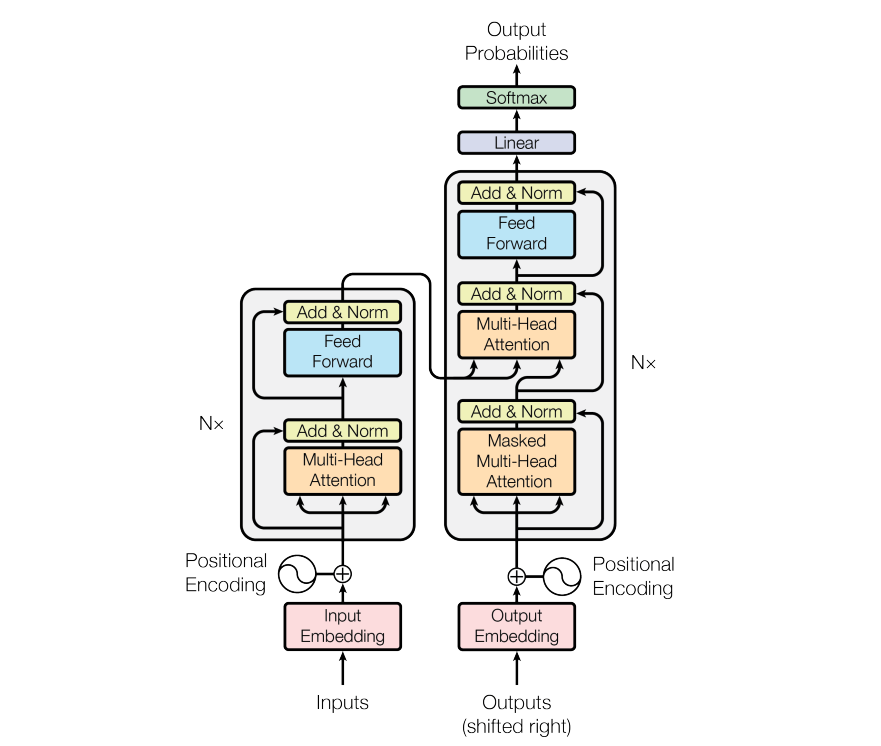
\includegraphics[width=0.9\linewidth]{figs/transformer.png}
  \caption{Transformerのアーキテクチャ\cite{vaswani2017attention}}
  \label{fig:tr_arch}
\end{figure}
\subsection{Vision Transformer}
Vision Transformerは,機械翻訳で用いられていたTransformerをコンピュータビジョンに適応させたモデルであり,画像を複数のパッチに分割してそれぞれをベクトルとして埋め込み,平坦化して入力とする特徴がある\cite{dosovitskiy2021image}.
Vision Transformerのアーキテクチャを\fref{fig:vit_arch}に示す.
\begin{figure}[H]
  \centering
  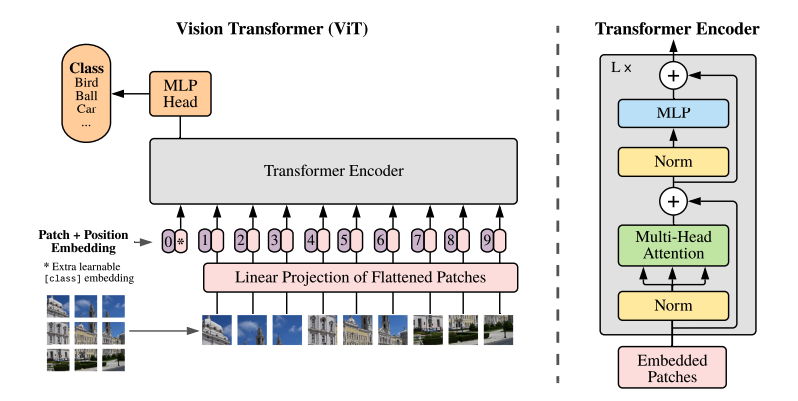
\includegraphics[width=0.9\linewidth]{figs/vit.png}
  \caption{Vision Transformerのアーキテクチャ\cite{dosovitskiy2021image}}
  \label{fig:vit_arch}
\end{figure}
\section{使用ツール・実験環境}
\subsection{Python}
Pythonは1990年代の始め,オランダにあるStichting Mathematisch CentrumでGuido van RossumによってABCと呼ばれる言語の後継言語として生み出された\cite{pythondoc}.
Pythonはコードを簡潔に書くことができ,数値計算のNumPy,データ解析のPandasなど,専門的なライブラリが充実していることから,機械学習の研究開発をはじめとしたさまざまな分野で使用されている言語である.
簡単にPythonを始めることができるディストリビューションとしてAnacondaがよく使われる.また,本実験で使用したバージョンは3.7.10である.
\subsection{PyTorch}
PyTorchはディープラーニング・プロジェクトの構築を容易にする,Pythonのライブラリである.柔軟性を重視した設計であり,さらに,ディープラーニングモデルをPythonの慣用的なクラスや関数の取り扱い方
で実装できるようになっている\cite{Eli_Stevens2021-01-30}.本実験で使用したバージョンは1.9.1である.
\subsection{Pytorch Image models}
Pytorch Image Models(timm)はRoss Wightmanによって作成されたディープラーニングライブラリであり,コンピュータビジョンの最先端のモデルが集められている\cite{timmdoc}.
数行の記述でモデルを呼び出すことができ,必要に応じて書き換えることで,さまざまなタスクに適用できる.本実験で使用したバージョンは0.5.2である.
\subsection{Albumentations}
AlbumentationsはPythonのためのデータ拡張のライブラリである.
モデルの汎化性能を上げるために行うデータ拡張のメソッドを多数揃えており,パイプラインを構成するとデータを効率的に拡張できる\cite{info11020125}.本実験で使用したバージョンは1.1.0である.
\subsection{ImageNet}
ImageNetはディープラーニング研究のために無償で利用できる大規模なデータセットのことで,モデルの性能を測るためのベンチマークとして使われる.
本実験ではImageNetの中でも「ILSVRC-2012 ImageNet」を使用する.このデータセットは,1,000のクラス,130万枚の画像で構成されている.
また,事前学習の規模によって認識精度が向上するViTの性質を確かめるために,より大規模なデータセットとして,ImageNet-21kを使用した.このデータセットは21,000のクラス及び1,400万枚の画像で構成されている.
\subsection{Kaggle}
Kaggleは世界規模のデータサイエンスのプラットフォームであり,世界中のデータサイエンティストが技術を競う場である.
本実験ではKaggleが提供しているNotebookのGPUを利用して学習及び推論を行う.
\subsection{Plant Pathology 2021 - FGVC8}
本実験ではKaggle上で提供されているコンペティションデータセットのPlant Pathology2021を用いる.
このコンペティションの目的はリンゴの葉の画像から,12の病気を正確に診断することである.
データセットの構成を\tref{tb:dataset}に,各病名とユニークな値にエンコードしたペアを\tref{tb:labels}に示す.
\begin{table}[H]
  \caption{データセットの構成}
  \label{tb:dataset}
  \centering\begin{tabular}{c|ccc}\hline
    データセットの構成 & 説明\\ \hline
    test\_images & 3枚の画像\\ \hline
    train\_images & 18,632枚の画像\\ \hline
    sample\_submission.csv & 提出用のサンプルcsvファイル\\ \hline
    train.csv & image,labelsの2カラムのcsvファイル\\ \hline
  \end{tabular}
\end{table}
\begin{table}[H]
  \caption{病名とユニークな値のペア}
  \label{tb:labels}
  \centering\begin{tabular}{c|ccc}\hline
    ユニークな値 & 病名\\ \hline
    0 & complex\\ \hline
    1 & frog\_eye\_leaf\_spot\\ \hline
    2 & frog\_eye\_leaf\_spot complex\\ \hline
    3 & healthy\\ \hline
    4 & powdery\_mildew\\ \hline
    5 & powdery\_mildew complex\\ \hline
    6 & rust\\ \hline
    7 & rust complex\\ \hline
    8 & rust frog\_eye\_leaf\_spot\\ \hline
    9 & scab\\ \hline
    10 & scab frog\_eye\_leaf\_spot\\ \hline
    11 & scab frog\_eye\_leaf\_spot complex\\ \hline
  \end{tabular}
\end{table}
%画像のラベル十二個を説明する

\section{論文の構成}
2章では実験に使用するモデルViTのアーキテクチャを数式を用いて説明し,実験の手順や条件について示す.3章では実験結果を図と表を用いて示す.
4章では3章の結果をもとに議論を行い,理解を深める.5章では今回の実験の総括を行う.

\chapter{実験モデル}

\section{ネットワークモデル}
ViTの入力は画像である.画像サイズを\textit{H},\textit{W},チャネル数を\textit{C}とすると,入力\textit{x}は\eref{eq:network-input1}のように表せる.
\begin{equation}
  x\in\mathbb{R}^{H\times W\times C}
  \label{eq:network-input1}
\end{equation}
また,二次元画像を扱うために,二次元の平坦化したパッチに整形する.\eref{eq:network-input2}に示す.
\begin{equation}
  x_{p}\in\mathbb{R}^{N\times(P^{2}\times C)}
  \label{eq:network-input2}
\end{equation}
ここで,\textit{N}はパッチ数であり,\textit{P}はパッチサイズである.また,\textit{N}は\textit{H},\textit{W},\textit{P}を用いて\eref{eq:network-input3}のように表せる.
\begin{equation}
  N=\frac{HW}{P^{2}}
  \label{eq:network-input3}
\end{equation}
ViTのエンコーダに入力するには,$x_{p}$をさらに埋め込む必要がある.長さ$P^{2}\times C$を\textit{D}次元のベクトルとして,線形投影したものを埋め込みパッチ$z_{0}$とする.
また,入力データの先頭には[class]トークンを付与し,埋め込みパッチ$z^{0}_{0}=x_{class}とする$.\eref{eq:network-input4}に示す.
\begin{equation}
  z_{0}=[x_{class};\ x^{1}_{p}E;\ x^{2}_{p}E;...;\ x^{N}_{p}E]+E_{pos},\qquad E\in\mathbb{R}^{(P^{2}\times C)\times D},\ E_{pos}\in\mathbb{R}^{(N+1)\times D}
  \label{eq:network-input4}
\end{equation}
ここで,\textit{E}はパッチを\textit{D}次元のベクトルへの埋め込みを示し,$E_{pos}$は各パッチの位置が一意に定まるように情報を付加する位置エンコーディングを表す.
上式で得られた入力$z_{0}$はMulti-Head Attentionに入力される.Multi-Head Attentionでは,Attentionを求める計算を複数回行う.具体的な算出については\ref{sec:attention}に示した.Attentionの算出式を\eref{eq:network-input5}に示す.
\begin{equation}
  Attention(Q,K,V) = softmax(\frac{QK^{T}}{\sqrt{d_{k}}})V
  \label{eq:network-input5}
\end{equation}
初めに,入力ベクトルから\textit{Q,K,V}ベクトルを生成する.このとき,\textit{Q,K}の次元は$d_{k}$で,\textit{V}の次元は$d_{k}$である.
計算時は,\textit{Q,K}の要素積を$\sqrt{d_{k}}$で割り,softmax関数で0から1の値に収め,総和を1にする.最後に\textit{V}をかけるとAttentionが算出できる.
Attentionの算出過程を\fref{fig:attention}に示す.
\begin{figure}[h]
  \centering
  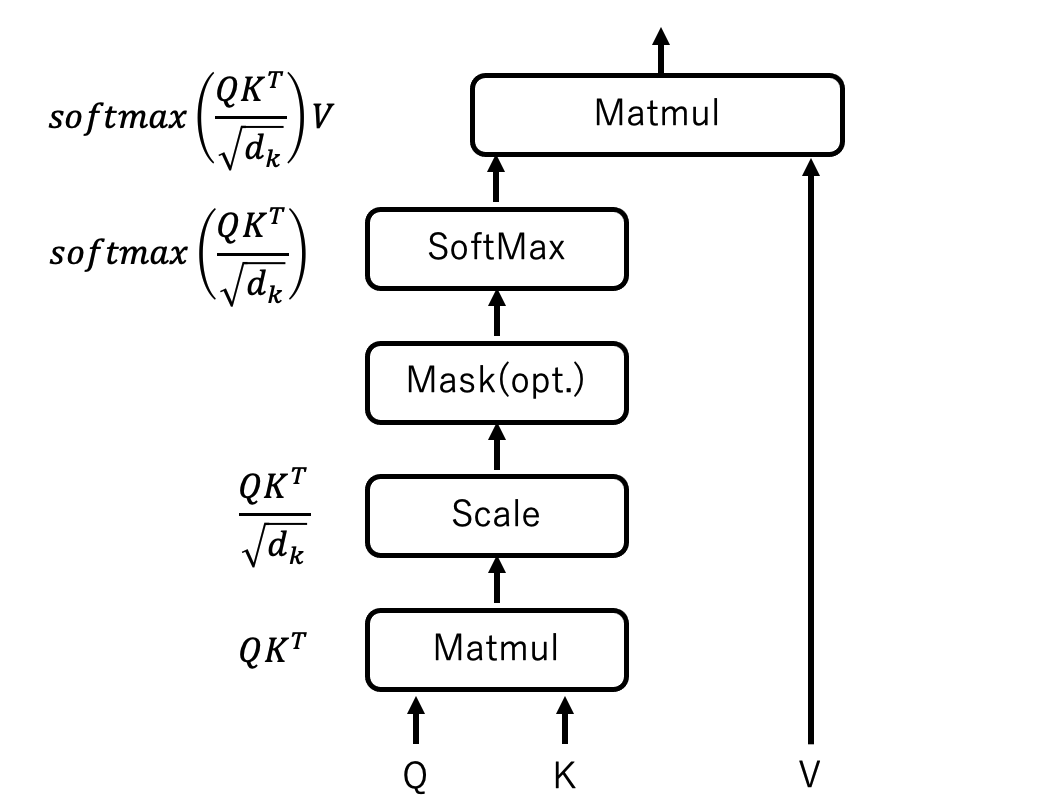
\includegraphics[width=0.9\linewidth]{figs/attention.png}
  \caption{Attentionの算出過程}
  \label{fig:attention}
\end{figure}

\section{評価指標}
本実験で使用するモデルの評価指標とその説明を以下に示す.
\subsection{Confusuion Matrix}
Confusuion Matrixは二値分類の正解及び不正解の種類を示す表のことであり,以下の4つの要素で構成されている.
\begin{enumerate}
  \item True Positive(TP) : 真陽性.正しく正例と判断.
  \item False Positive (FP): 偽陽性.誤って正例と判断.
  \item True Negative (TN): 真陰性.正しく負例と判断.
  \item False Negative (FN): 偽陰性.誤って負例と判断.
\end{enumerate}

\subsection{Accuracy}
Accuracyは正解率ともいい,Confusion Matrixを用いて\eref{eq:acc_eq}と表せる.
\begin{equation}
  Accuracy=\frac{TP+TN}{TP+FP+TN+FN}
  \label{eq:acc_eq}
\end{equation}
予測した値のうち,正しく正例及び負例を予測できた割合を表し,得られる値は0から1をとり,1に近いほど良いスコアである.

\subsection{F1-Score}
F1-Scoreは,PrecisionとRecallの調和平均で計算される指標である,PresisionとRecallはConfusion Matrixを用いて\eref{eq:f1_eq}で表せる.
\begin{equation}
  Presision=\frac{TP}{TP+FP}\ Recall=\frac{TP}{TP+FN}
  \label{eq:f1_eq}
\end{equation}
Presisionは正例と予測したもののうち真の値も正例の割合,Recallは真の値が正例のもののうちどの程度を正例の予測として含めることができているかの割合である\cite{門脇大輔2019-10-09}.
また,これらはトレードオフの関係になっており,どちらかの値を高くしようとするともう一方の値は低くなる.そしてPresisionとRecallのバランスをとった指標がF1-Scoreである.\eref{eq:f1_eq2}に示す.
\begin{equation}
  F1-Score=\frac{2}{\frac{1}{Recall}+\frac{1}{Presision}}=\frac{2・Recall・Presicion}{Recall・Presicion}=\frac{2TP}{2TP+FP+FN}
  \label{eq:f1_eq2}
\end{equation}
また,F1-Scoreは二値分類における評価指標であり,他クラス分類に拡張したものに,mean-F1,macro-F1,micro-F1がある.本実験ではmacro-F1 Scoreを用いる.
macro-F1 ScoreはラベルごとにF1-Scoreを求め,それらの平均値を評価のスコアとする.

\subsection{Cross Entropy Loss \cite{torchdoc}}
Cross Entropy Lossの算出式は\eref{eq:loss_eq}で示される.%\sum_{n = 1}^{\infty}
\begin{equation}
  Loss(x,class)=-\rm{log}\Biggl(\frac{\exp(\textit{x}[\textit{class}])}{\sum_{\textit{j}=0}^{\textit{n}-1}\rm{exp}(\textit{x}[\textit{j}])}\Biggr)=-\textit{x}[\textit{class}]+log\Biggl(\sum_{\textit{j}=0}^{\textit{n}-1}exp(\textit{x}[\textit{j}])\Biggr)
  \label{eq:loss_eq}
\end{equation}
ここで,\textit{x}はモデルからの出力(予測),\textit{class}は正解ラベル,\textit{n}はクラス数を示す.
例えば,$x=[-1.6059,-0.1475,-0.3950,-0.8846]$,$class=1$,$\textit{n}=4$とする.この場合のCross Entropy Lossは\eref{eq:loss_eq2}のように算出される.
\begin{equation}
  \begin{split}
    Loss&=-\textit{x}[\textit{class}]+\rm{log}\Biggl(\sum_{\textit{j}=0}^{\textit{n}-1}exp(\textit{x}[\textit{j}])\Biggr)\\
    &=-x[1]+\rm{log}\Bigl(\rm{exp}(x[0])+\rm{exp}(x[1])+\rm{exp}(x[2])+\rm{exp}(x[3])\Bigr)\\
    &=0.1475+\rm{log}(2.1501)\\
    &=0.9130\\
  \end{split}
  \label{eq:loss_eq2}
\end{equation}

\section{手順}
実験の条件を\tref{tb:conditions}に示す.
\begin{table}[htbp]
  \caption{実験の条件}
  \label{tb:conditions}
  \centering\begin{tabular}{c|cccc}\hline
    \backslashbox{条件}{オプション} & 事前学習 & データ拡張 & ILSVRC-2012 ImageNet & ImageNet-21k\\\hline
    条件1 & なし & なし & $\circ$ & $\times$\\\hline
    条件2 & あり & なし & $\circ$ & $\times$\\\hline
    条件3 & あり & あり & $\circ$ & $\times$\\\hline
    条件4(ViTのみ) & あり & あり & $\circ$ & $\circ$\\\hline
  \end{tabular}
\end{table}

実験手順を以下に示す.

\begin{enumerate}
  \item 条件1では,事前学習・データ拡張を行わなずに認識精度を検証する.論文より\cite{dosovitskiy2021image},ViTは大規模なデータセットで事前学習を行なった場合に良い認識精度を発揮することがわかっているので,
以降,このスコアを一つの基準として比較を進める.
  \item 条件2では,事前学習を行い,データ拡張は行わない.予想される結果として,訓練データにオーバーフィッティングすることが考えられる.
  \item 条件3では,オーバーフィッティングを防ぎ,検証データに対して認識精度を向上させるために,データ拡張を行う.これにより,訓練時と検証時の各指標の差異が小さくなると考えられる.
  また,今回の実験で使用したデータ拡張はResize,Rotate,Horizontal Flip,Grid Dropout,Brightness Contrastである.それぞれ\fref{fig:aug}に示す.
  \begin{figure}[H]
    \begin{tabular}{cc}
      \begin{minipage}[t]{0.45\hsize}
        \centering
        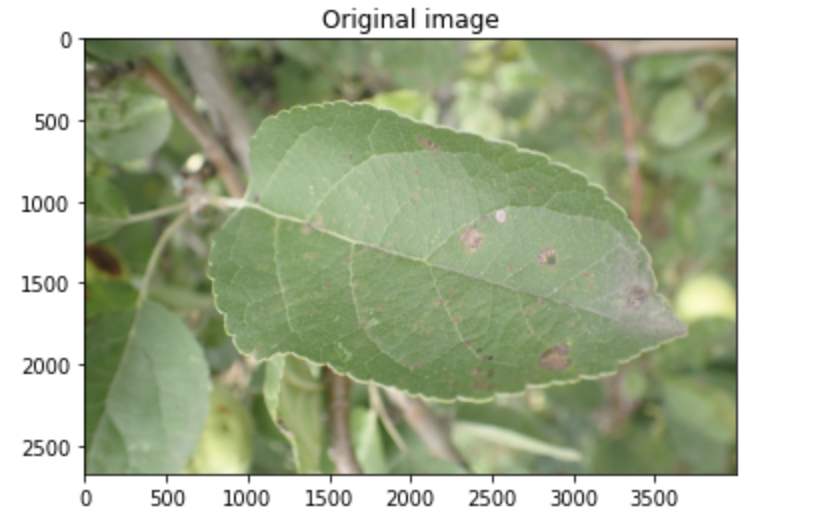
\includegraphics[keepaspectratio, scale=0.43]{figs/original.png}
        \subcaption{Original}
        %\label{Accuracy}
      \end{minipage} &
      \begin{minipage}[t]{0.45\hsize}
        \centering
        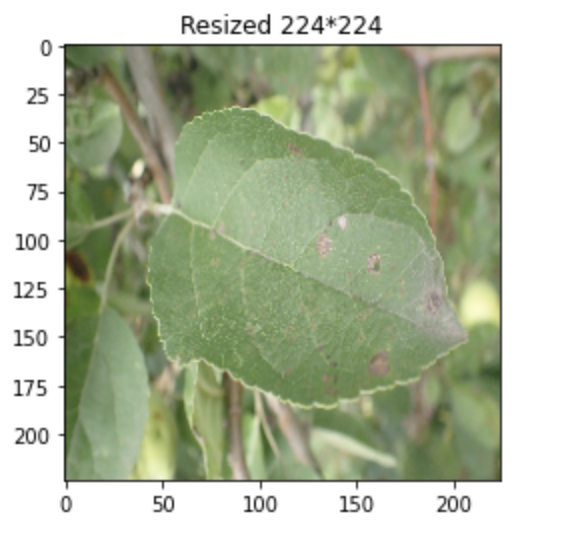
\includegraphics[keepaspectratio, scale=0.43]{figs/resize.png}
        \subcaption{Resize}
        %\label{F1-Score}
      \end{minipage} \\
  
      \begin{minipage}[t]{0.45\hsize}
        \centering
        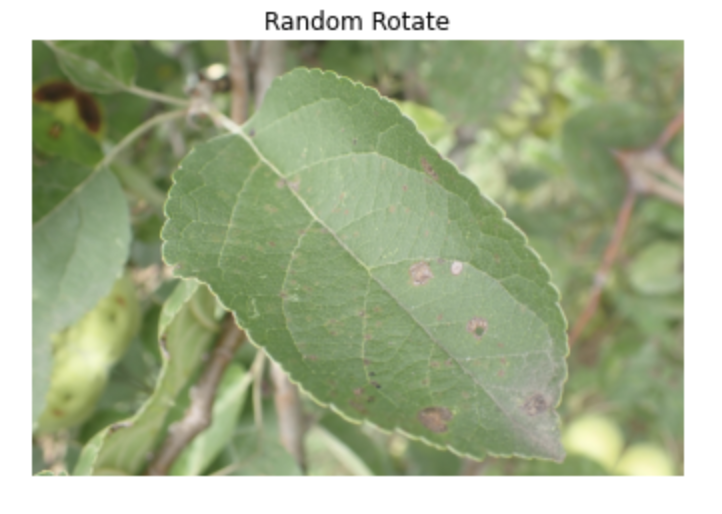
\includegraphics[keepaspectratio, scale=0.43]{figs/random_rotate.png}
        \subcaption{Rotate}
        %\label{Loss}
      \end{minipage} &
      \begin{minipage}[t]{0.45\hsize}
        \centering
        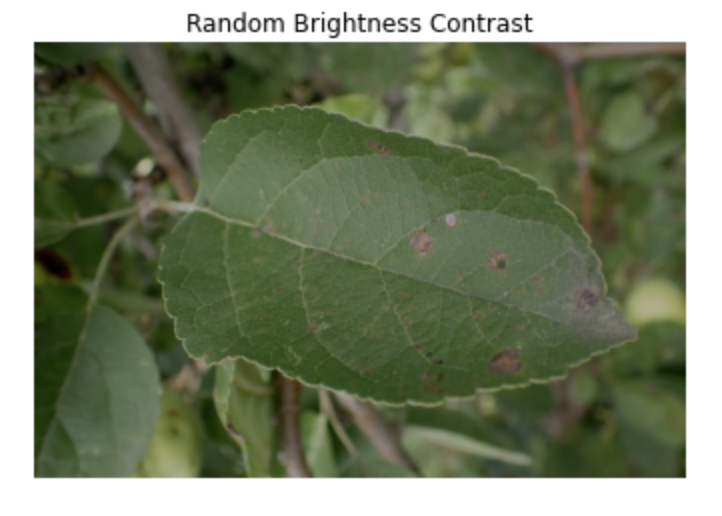
\includegraphics[keepaspectratio, scale=0.43]{figs/random_brightness_contrast.png}
        \subcaption{Brightness Contrast}
        %\label{Loss}
      \end{minipage} \\

      \begin{minipage}[t]{0.45\hsize}
        \centering
        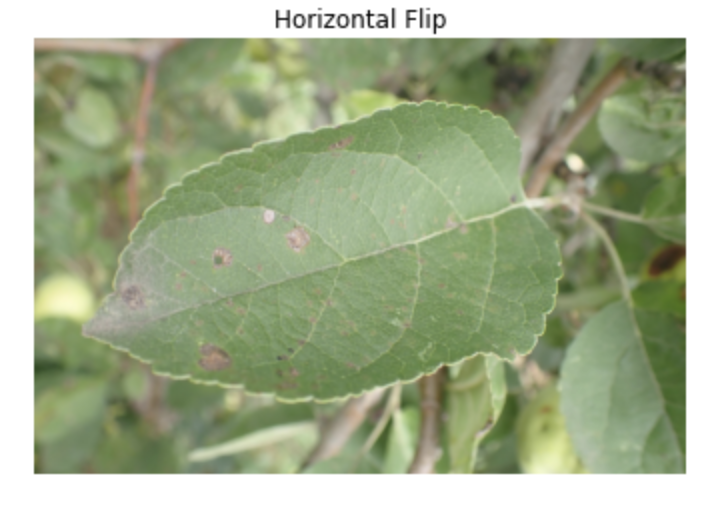
\includegraphics[keepaspectratio, scale=0.43]{figs/holizontal_flip.png}
        \subcaption{Horizontal Flip}
        %\label{Loss}
      \end{minipage} &
      \begin{minipage}[t]{0.45\hsize}
        \centering
        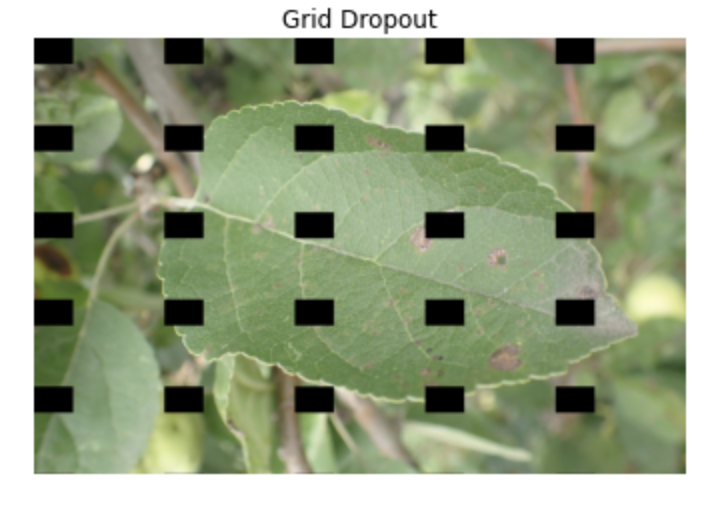
\includegraphics[keepaspectratio, scale=0.43]{figs/grid_dropout.png}
        \subcaption{Grid Dropout}
        %\label{Loss}
      \end{minipage}
    \end{tabular}
    \caption{条件1の実験結果}
    \label{fig:aug}
  \end{figure}
  \item 条件4では,ViTのみで実験を行う.先に述べた通り,ViTは事前学習の規模が大きいほど各画像認識のベンチマークで良い認識結果が得られている.そこで,条件3までで事前学習に使用してきたデータセットのILSVRC-2012 ImageNetに加え,
  より規模の大きいImageNet-21kを使用する.これにより各指標がこれまでよりいい結果を示すと予想される.
\end{enumerate}
\subsection{モデルのパラメータ}
本実験で使用した各モデルのパラメータ及び設定を\tref{tb:param}に示す.
\begin{table}[htbp]
  \caption{各モデルのパラメータ及び設定}
  \label{tb:param}
  \centering\begin{tabular}{c|ccc}\hline
    \backslashbox{設定}{モデル} & vit\_base\_patch\_224 & resnet18d & vgg11\\\hline
    image size & 224x224 & 224x224 & 224x224\\\hline
    batch size & 32 & 32 & 32\\\hline
    debug size & 0.2 & 0.2 &0.2\\\hline
    epoch & 10 & 10 & 10\\\hline
    learning rate & 1e-4 & 1e-4 &1e-4\\\hline
    optimizer & Adam(条件4のみSGD) & Adam & Adam\\\hline
    criterion & Cross Entropy Loss & Cross Entropy Loss & Cross Entropy Loss\\\hline
  \end{tabular}
\end{table}

\subsection{Optimizer SGD}
SGD(Stochastic Gradient Decent : 確率的勾配降下法)は代表的な最適化手法の一つで,求めた勾配方向にパラメータを更新する手法である\cite{斎藤康毅2016-09-24}.
パラメータの更新式を\eref{eq:sgd_eq}に示す.
\begin{equation}
  W\leftarrow W - \eta\frac{\partial L}{\partial W}
  \label{eq:sgd_eq}
\end{equation}
ここで,\textit{W}は更新する重みパラメータを表し,$\frac{\partial L}{\partial W}$は\textit{W}に関する損失関数\textit{L}の勾配である.
また,$\eta$は学習率であり,本実験では1e-4とした.

\subsection{Optimizer Adam}
Adamは,パラメータの要素ごとに適応的に学習率を調整しながら学習を行うAdaGrad \cite{斎藤康毅2016-09-24}と,過去の勾配を徐々に忘れて新しく求めた勾配を大きく反映させるRMSPropを組み合わせた手法である\cite{kingma2017adam}.
また,学習率の初期値は1e-4とした.
%理論難しい,要相談
\chapter{実験結果}

条件ごとの実験結果を\tref{tb:result1},\tref{tb:result2},\tref{tb:result3},\tref{tb:result4}に,
また,それに対応するグラフを\fref{fig:re1},\fref{fig:re2},\fref{fig:re3},\fref{fig:re4}に示す.
\newpage
\begin{table}[htbp]
  \caption{条件1の実験結果}
  \label{tb:result1}
  \centering\begin{tabular}{c|ccc}\hline
    \backslashbox{指標}{モデル} & vit\_base\_patch\_224 & resnet18d & vgg11\\\hline
    best valid accuracy & 0.5906 & 0.8209 & 0.8384\\\hline
    best valid f1-Score & 0.4453 & 0.6283 &0.6349\\\hline
    best valid loss & 1.1983 & 0.5554 &0.5132\\\hline
  \end{tabular}
\end{table}

%条件1の各指標の結果を\fref{fig:re1}に示す.
\begin{figure}[H]
  \begin{tabular}{cc}
    \begin{minipage}[t]{0.45\hsize}
      \centering
      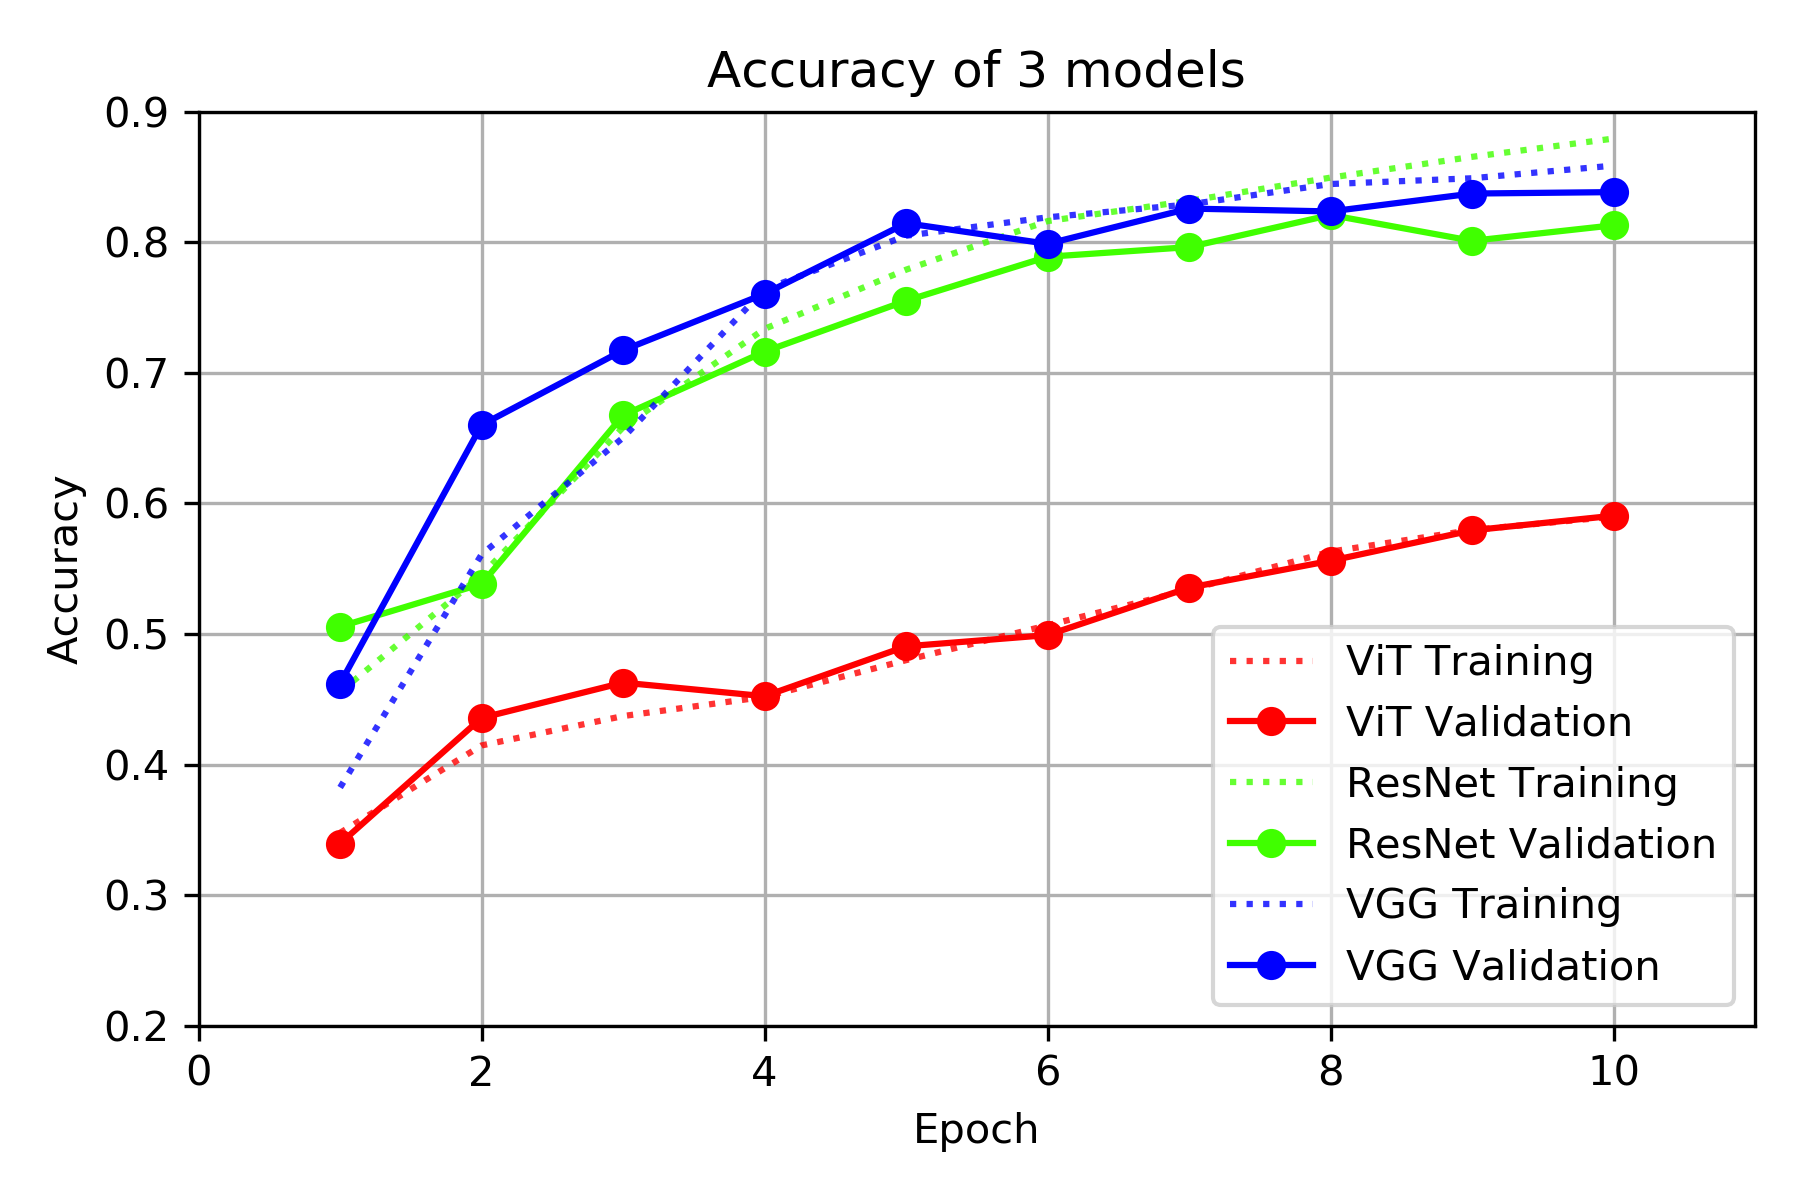
\includegraphics[keepaspectratio, scale=0.43]{figs/result1-1.png}
      \subcaption{Accuracy}
      %\label{Accuracy}
    \end{minipage} &
    \begin{minipage}[t]{0.45\hsize}
      \centering
      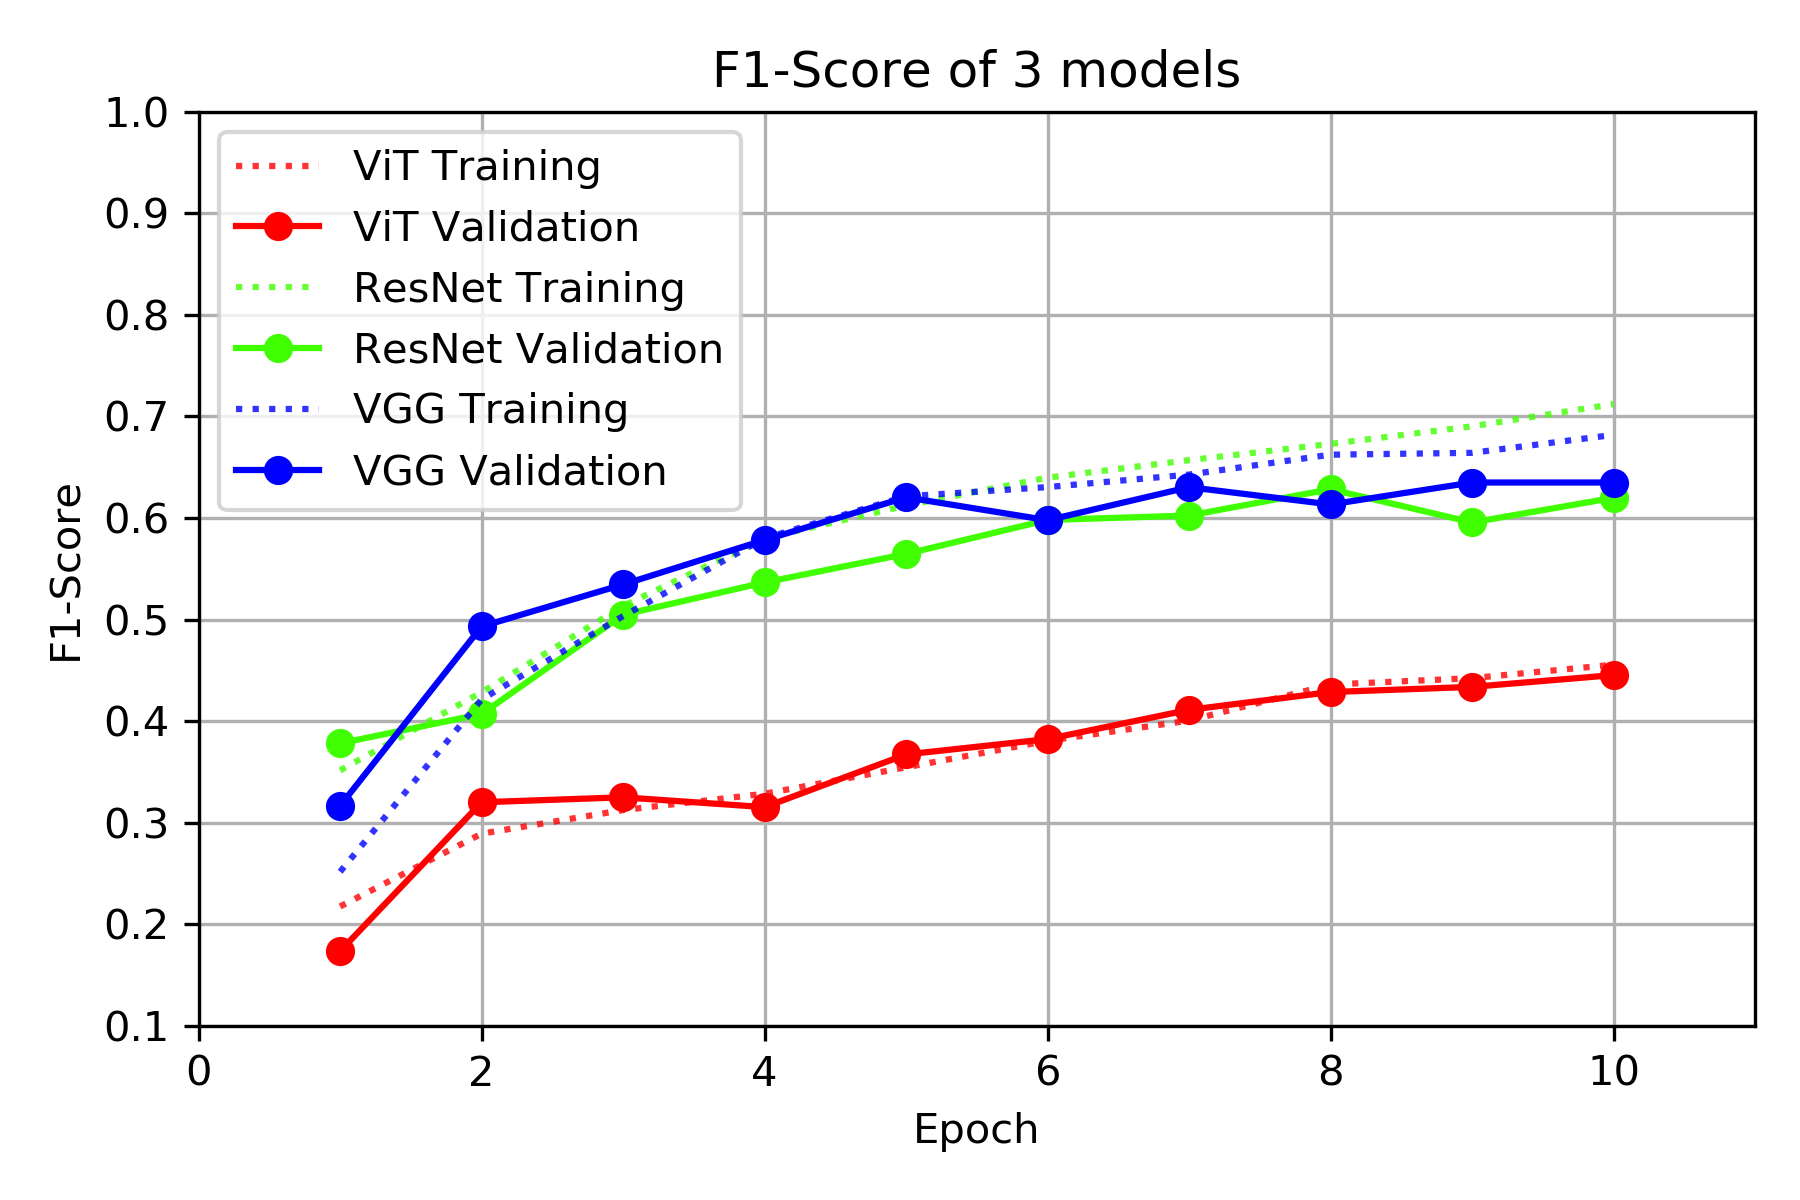
\includegraphics[keepaspectratio, scale=0.43]{figs/result1-2.png}
      \subcaption{F1-Score}
      %\label{F1-Score}
    \end{minipage} \\

    \begin{minipage}[t]{0.45\hsize}
      \centering
      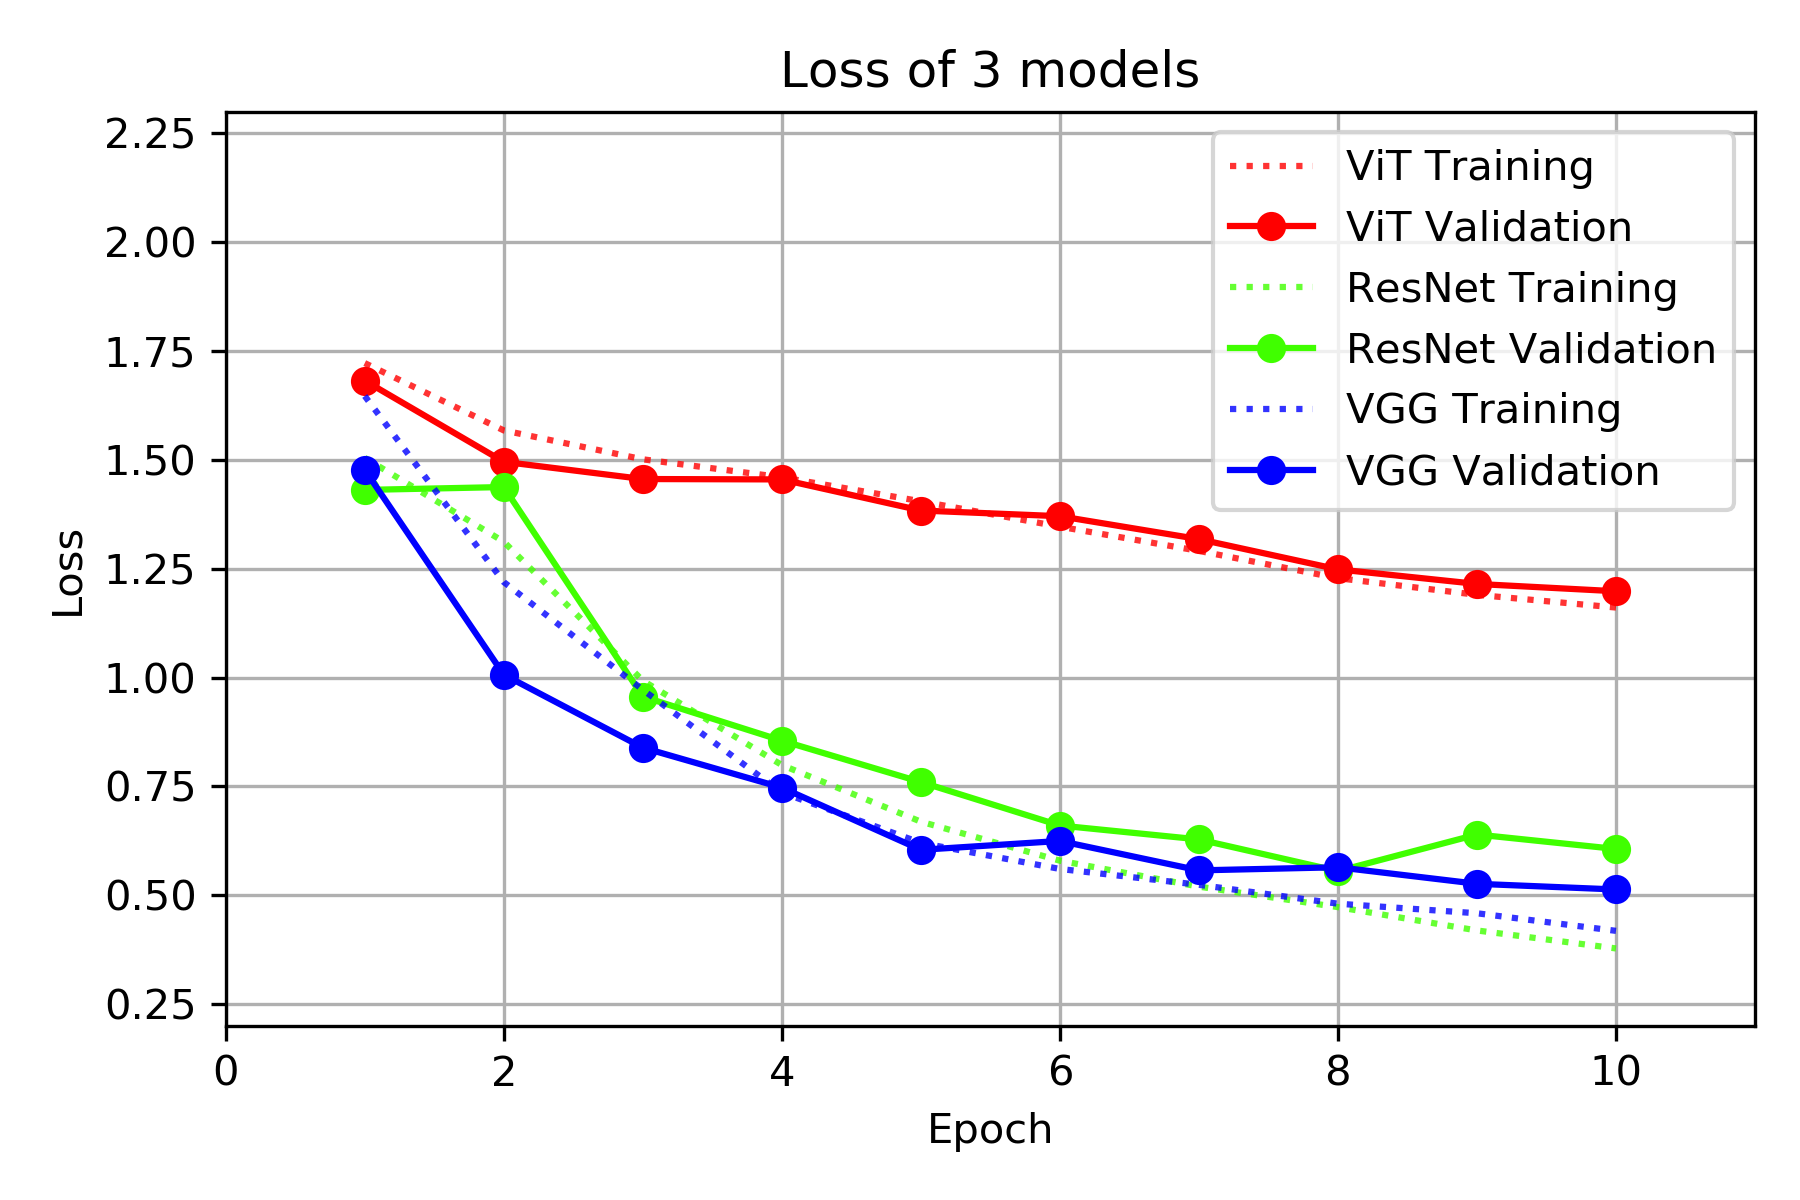
\includegraphics[keepaspectratio, scale=0.43]{figs/result1-3.png}
      \subcaption{Loss}
      %\label{Loss}
    \end{minipage}
  \end{tabular}
  \caption{条件1の実験結果}
  \label{fig:re1}
\end{figure}
\newpage
\begin{table}[htbp]
  \caption{条件2の実験結果}
  \label{tb:result2}
  \centering\begin{tabular}{c|ccc}\hline
    \backslashbox{指標}{モデル} & vit\_base\_patch\_224 & resnet18d & vgg11\\\hline
    best valid accuracy & 0.8312 & 0.8568 & 0.8611\\\hline
    best valid f1-Score & 0.6605 & 0.6708 &0.6798\\\hline
    best valid loss & 0.5562 & 0.4989 &0.4433\\\hline
  \end{tabular}
\end{table}

%条件2の各指標の結果を\fref{fig:re2}に示す.
\begin{figure}[H]
  \begin{tabular}{cc}
    \begin{minipage}[t]{0.45\hsize}
      \centering
      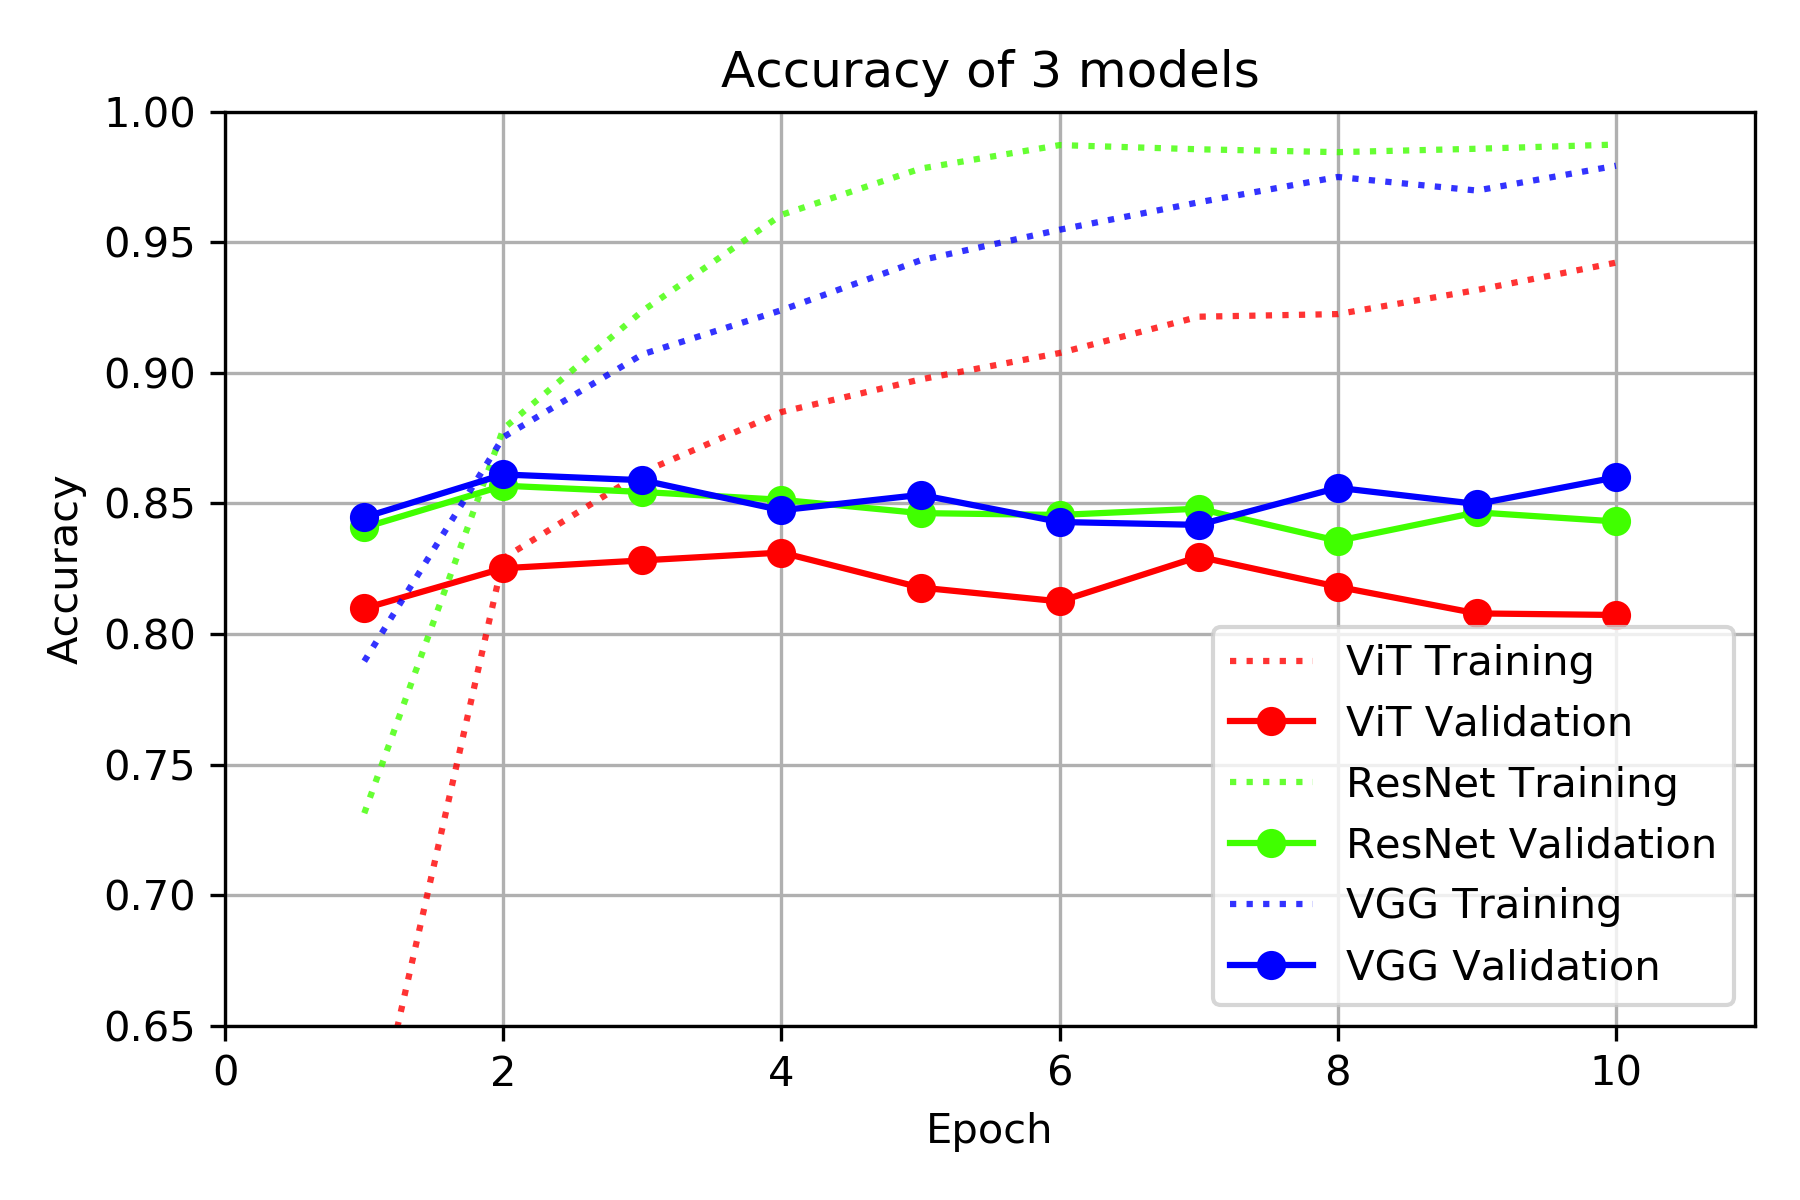
\includegraphics[keepaspectratio, scale=0.42]{figs/result2-1.png}
      \subcaption{Accuracy}
      %\label{composite}
    \end{minipage} &
    \begin{minipage}[t]{0.45\hsize}
      \centering
      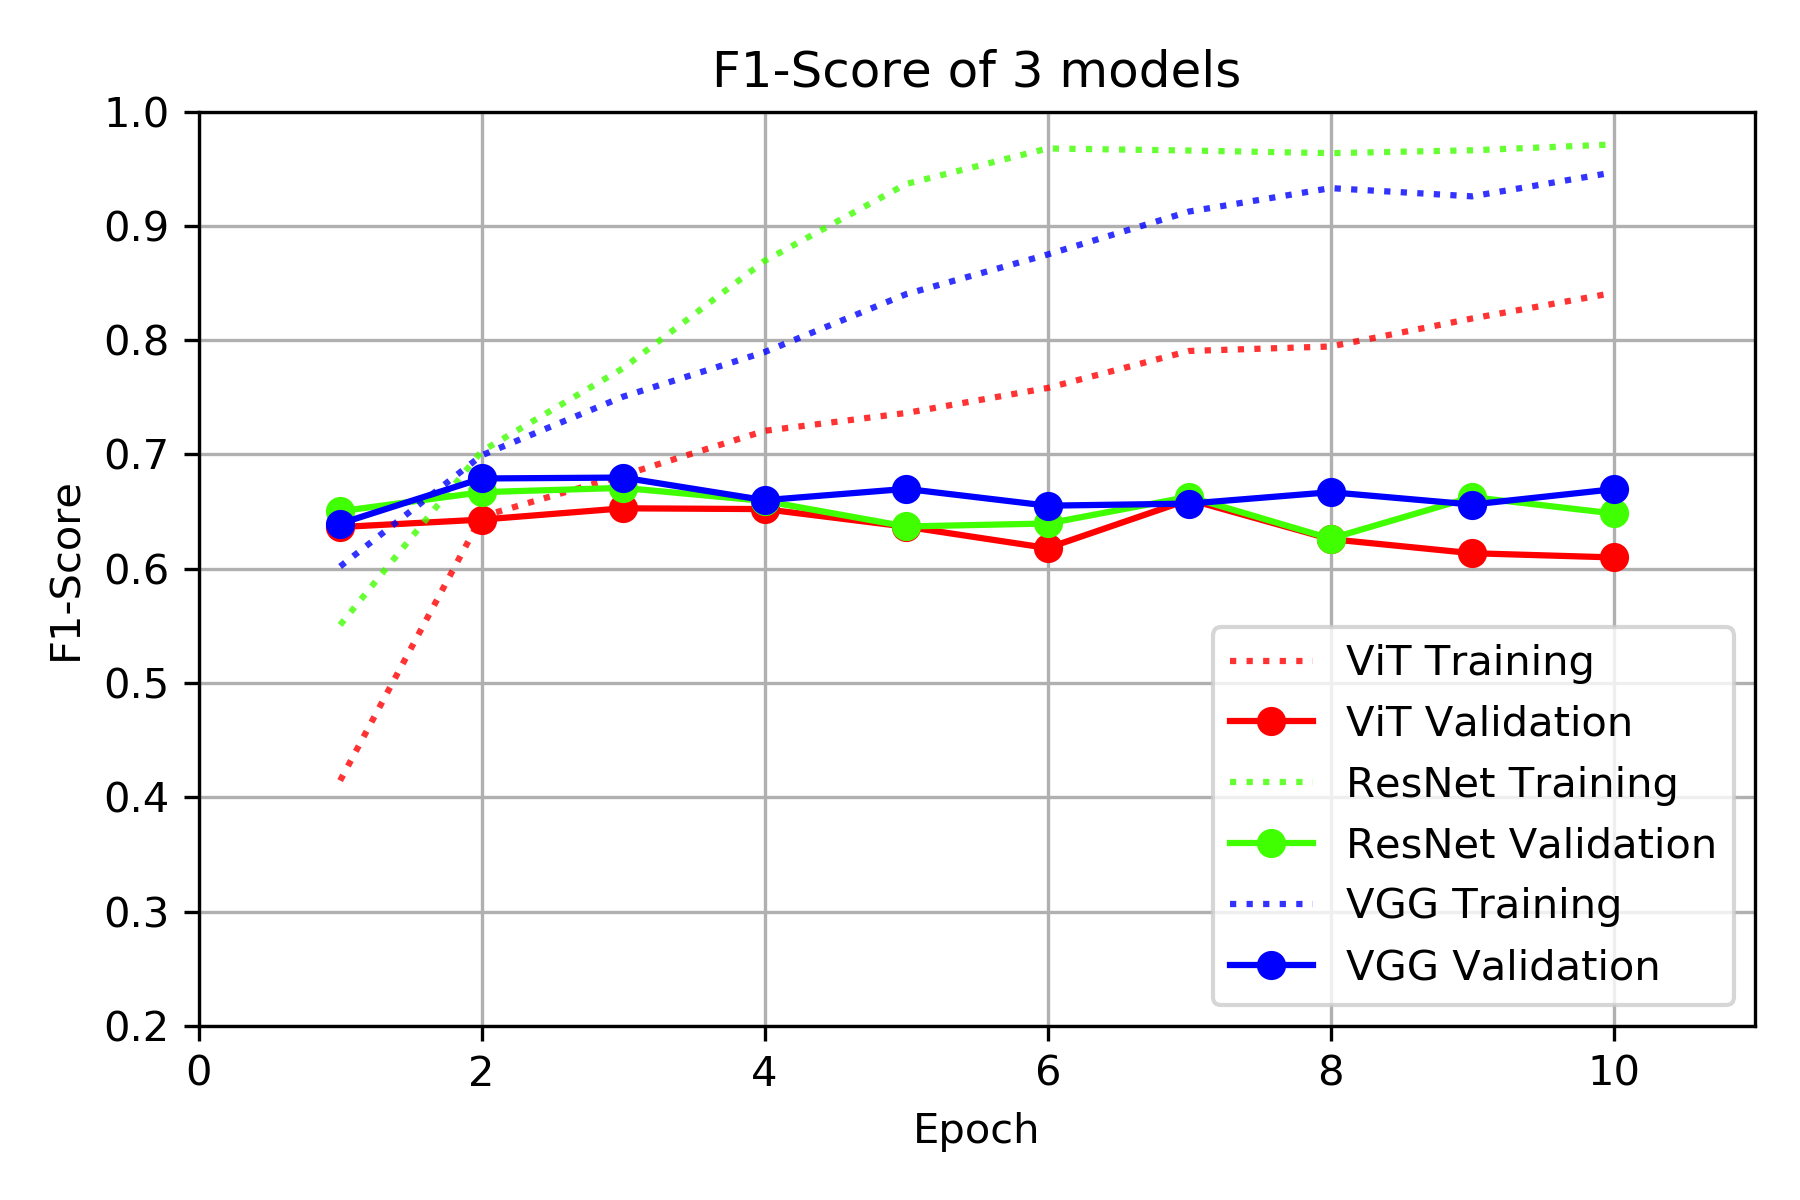
\includegraphics[keepaspectratio, scale=0.42]{figs/result2-2.png}
      \subcaption{F1-Score}
      %\label{Gradation}
    \end{minipage} \\

    \begin{minipage}[t]{0.45\hsize}
      \centering
      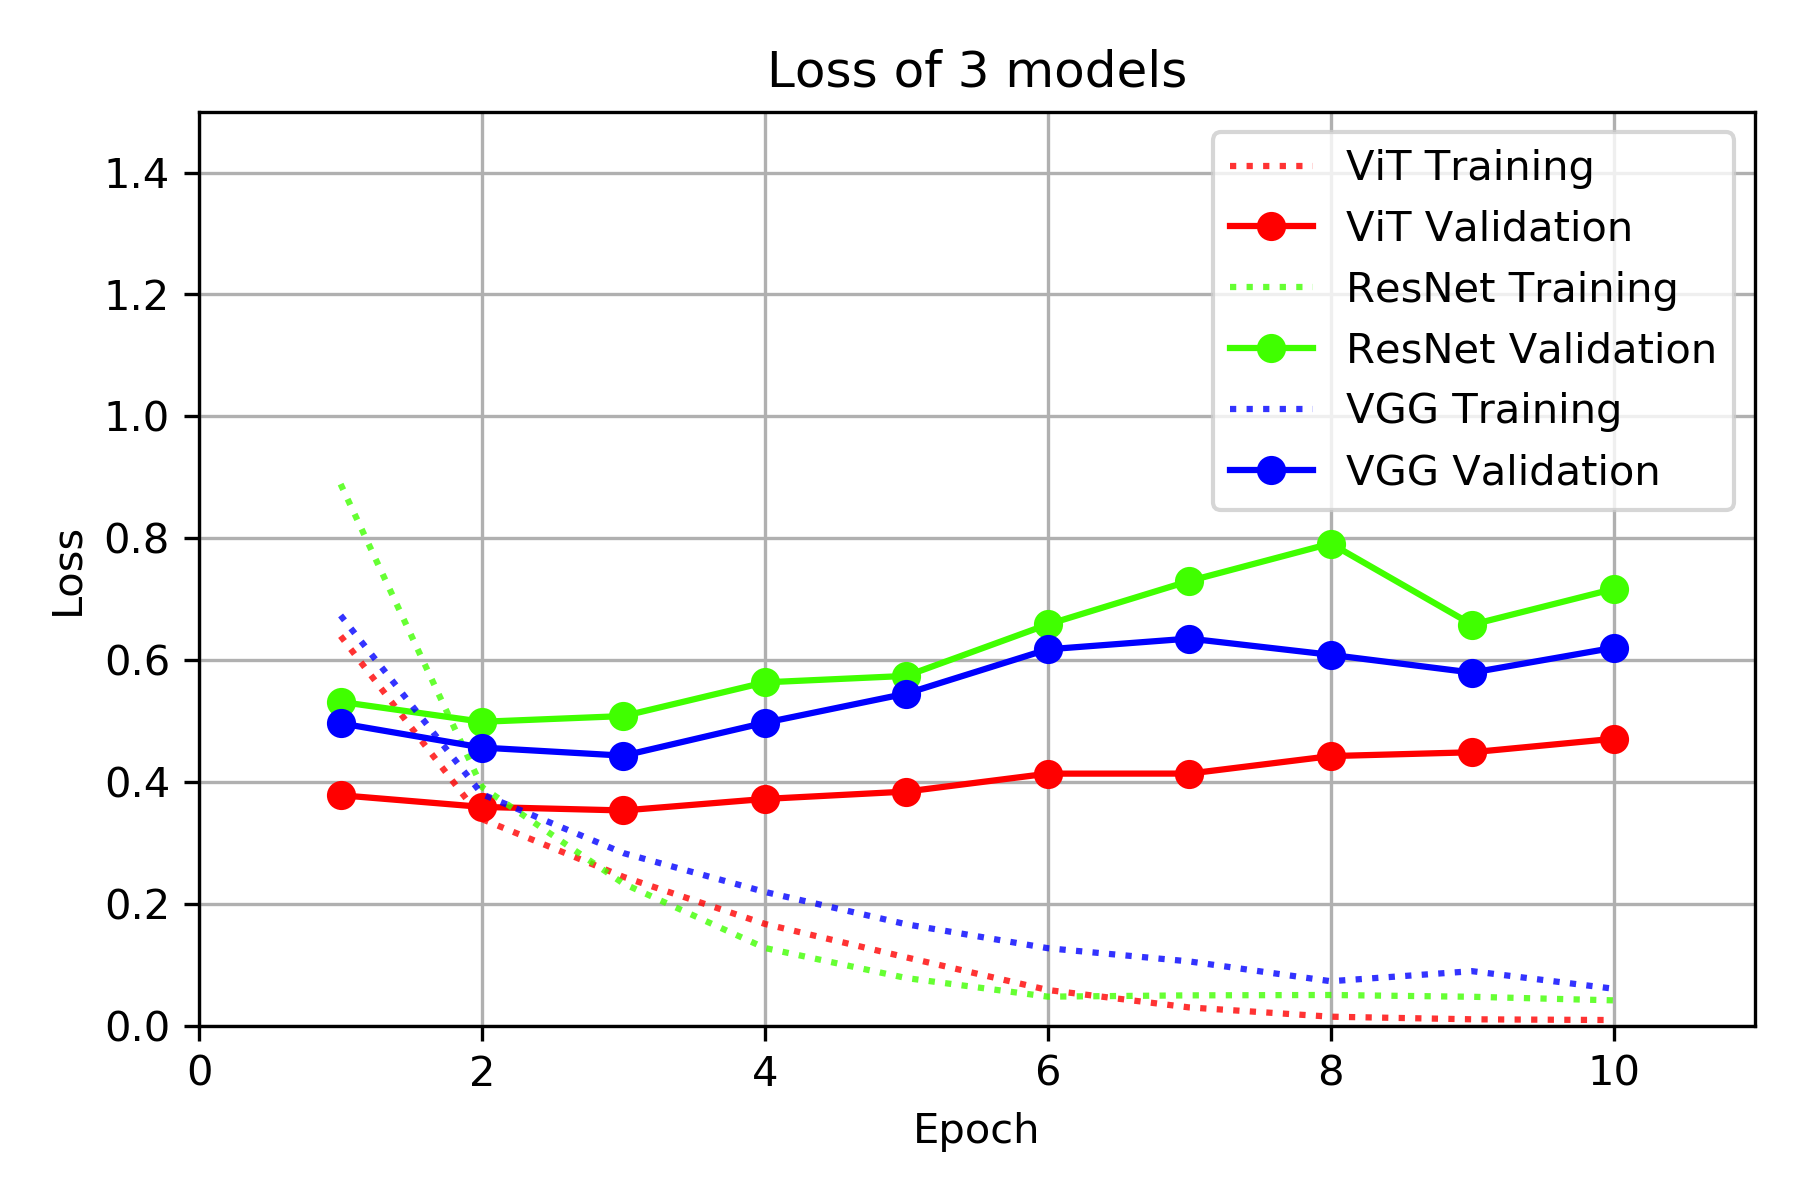
\includegraphics[keepaspectratio, scale=0.42]{figs/result2-3.png}
      \subcaption{Loss}
      %\label{fill}
    \end{minipage}
  \end{tabular}
  \caption{条件2の実験結果}
  \label{fig:re2}
\end{figure}
\newpage
\begin{table}[htbp]
  \caption{条件3の実験結果}
  \label{tb:result3}
  \centering\begin{tabular}{c|ccc}\hline
    \backslashbox{指標}{モデル} & vit\_base\_patch\_224 & resnet18d & vgg11\\\hline
    best valid accuracy & 0.8806 & 0.8881 & 0.8856\\\hline
    best valid f1-Score & 0.7199 & 0.7141 &0.7114\\\hline
    best valid loss & 0.3809 & 0.3626 &0.3635\\\hline
  \end{tabular}
\end{table}
%条件3の各指標の結果を\fref{fig:re3}に示す.
\begin{figure}[H]
  \begin{tabular}{cc}
    \begin{minipage}[t]{0.45\hsize}
      \centering
      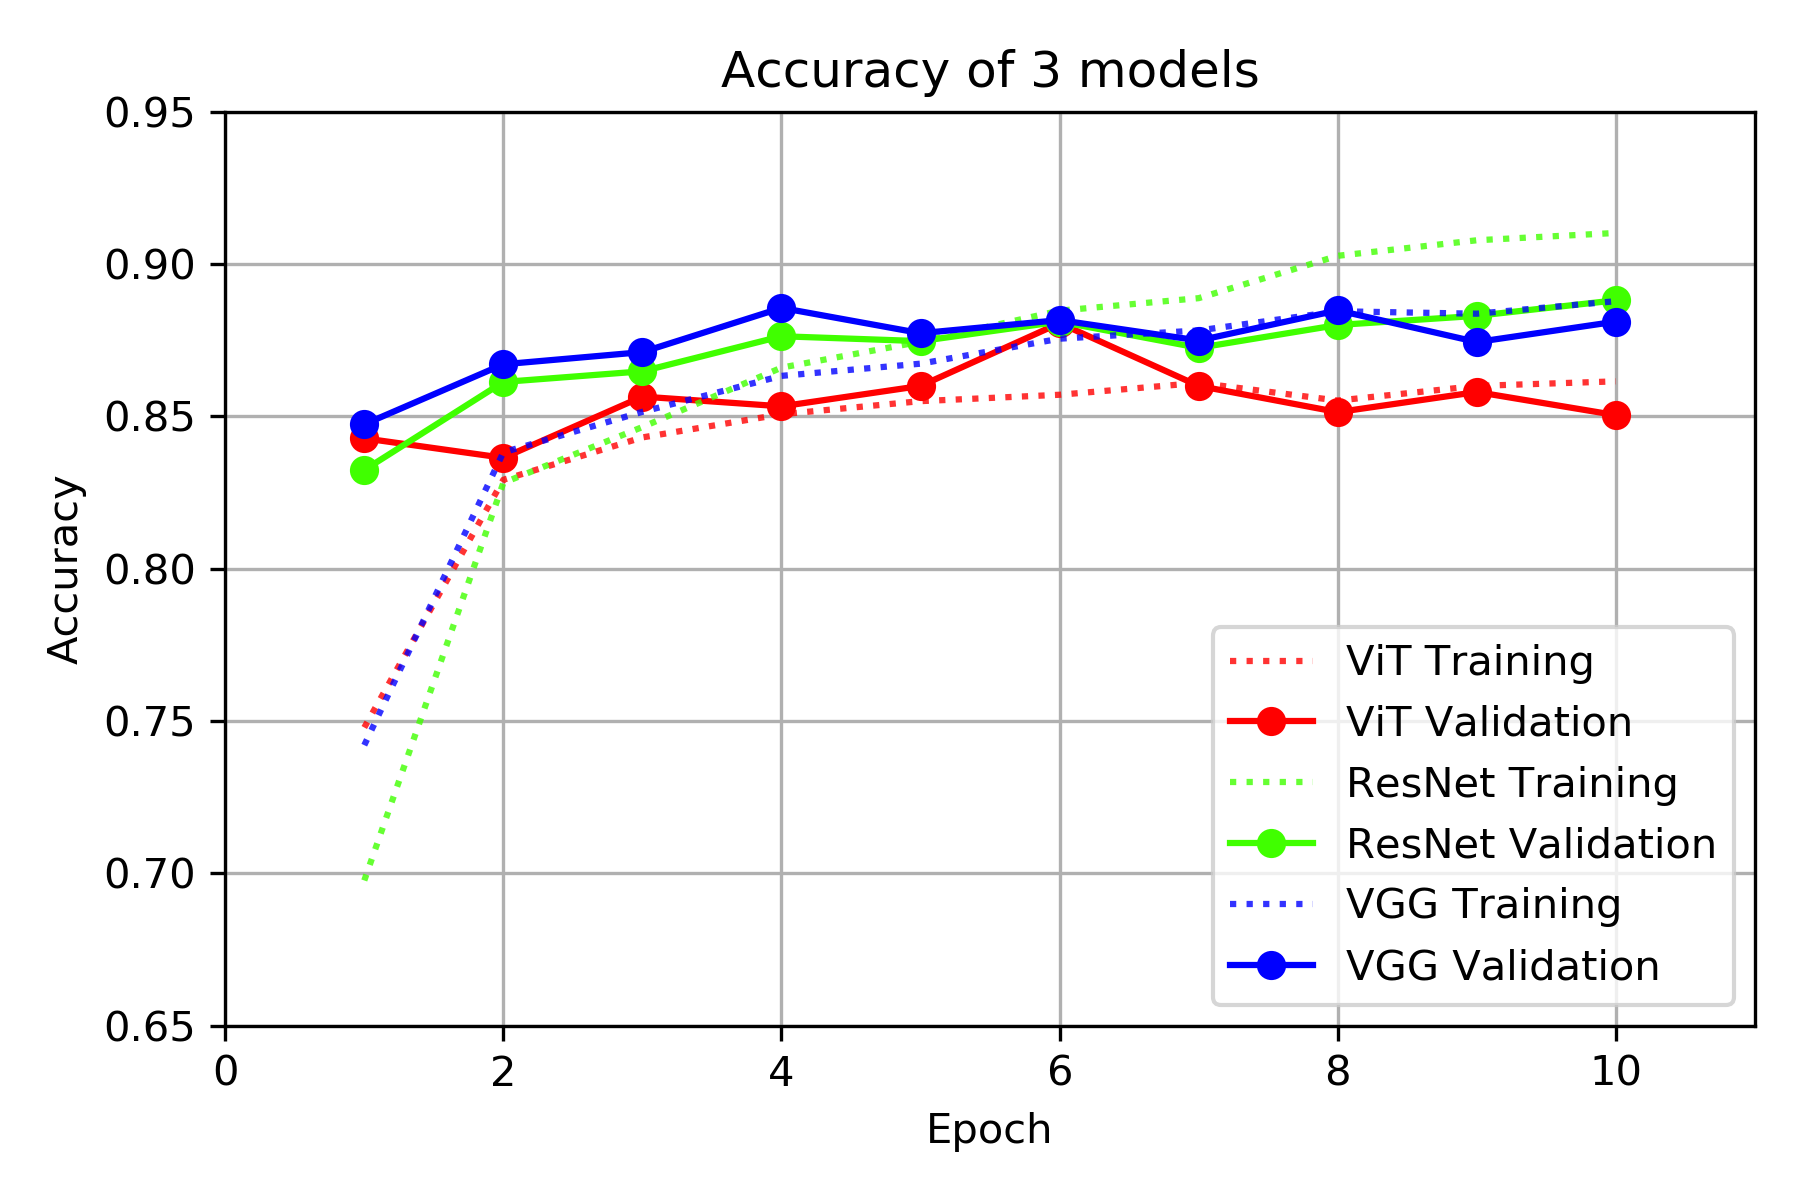
\includegraphics[keepaspectratio, scale=0.43]{figs/result3-1.png}
      \subcaption{Accuracy}
      %\label{composite}
    \end{minipage} &
    \begin{minipage}[t]{0.45\hsize}
      \centering
      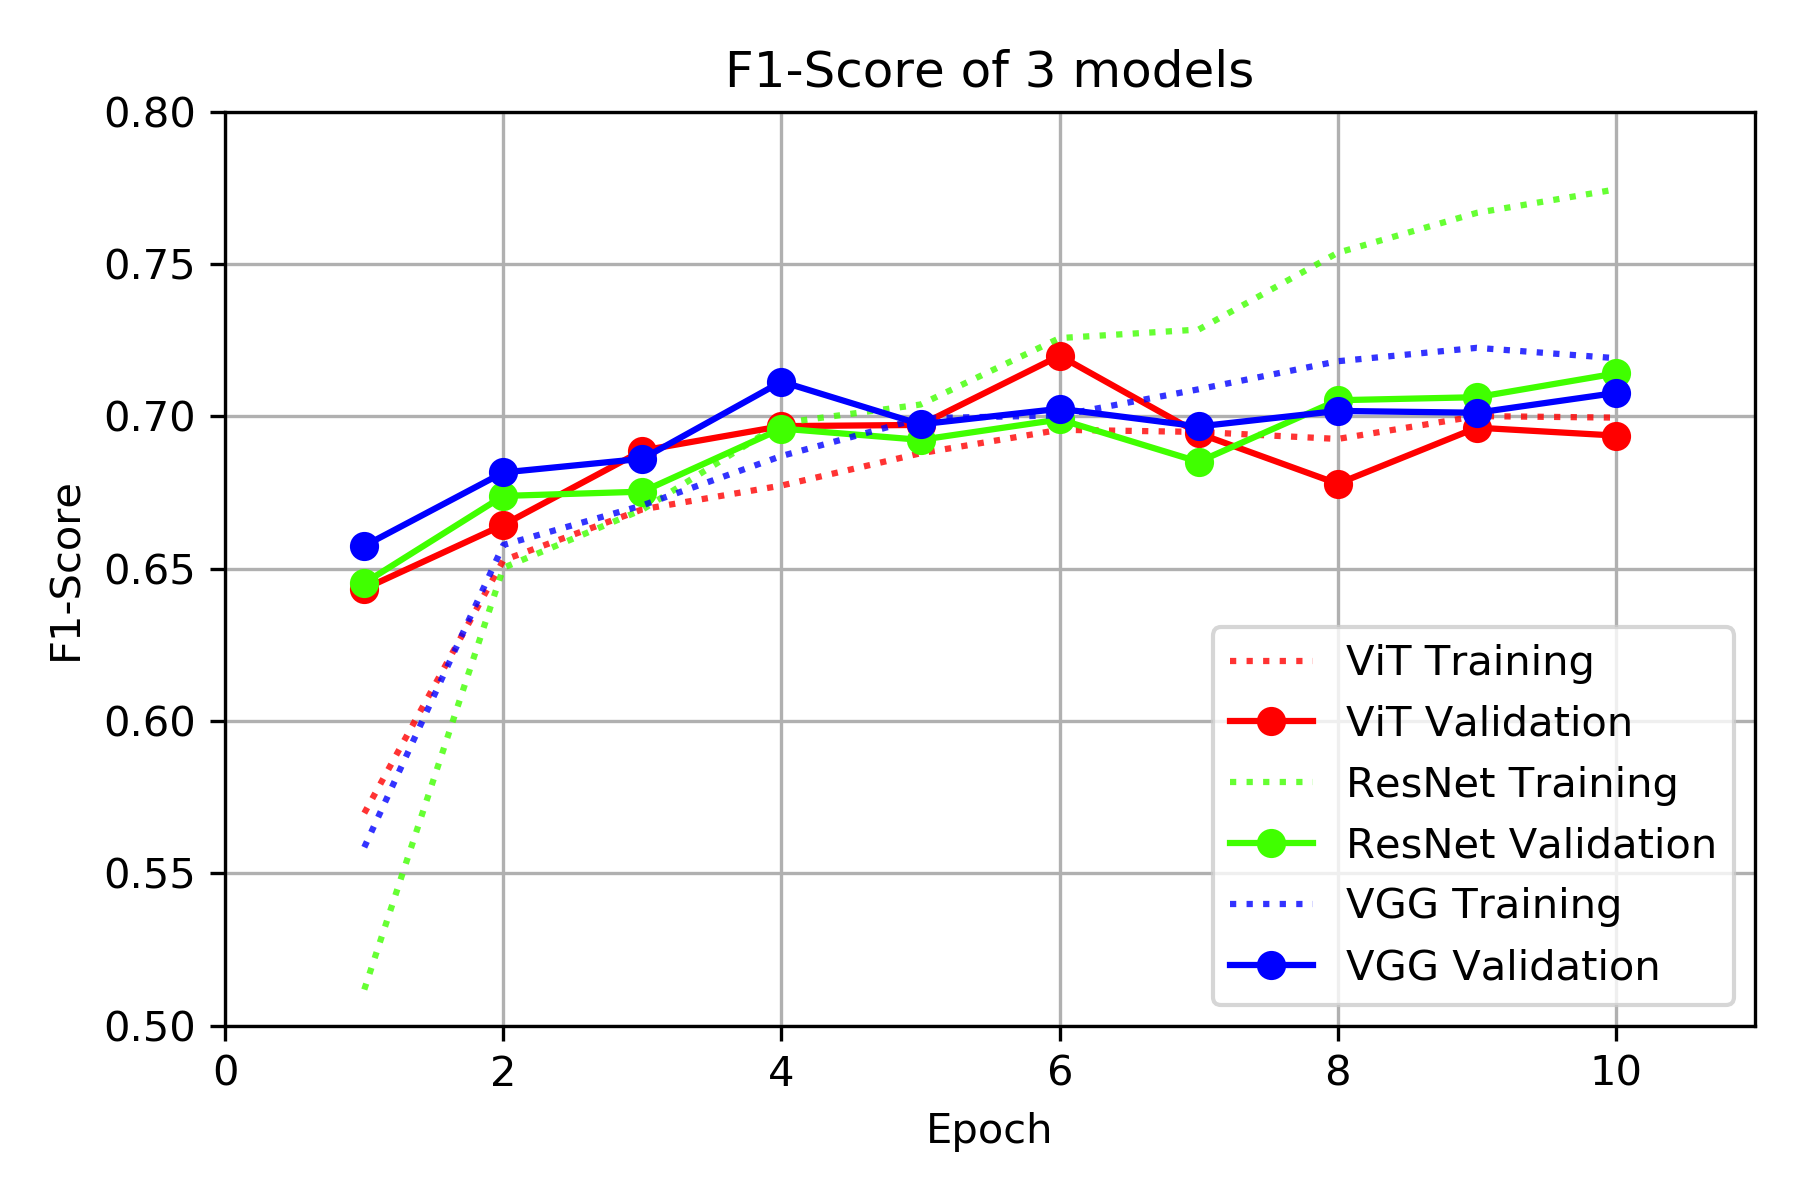
\includegraphics[keepaspectratio, scale=0.43]{figs/result3-2.png}
      \subcaption{F1-Score}
      %\label{Gradation}
    \end{minipage} \\

    \begin{minipage}[t]{0.45\hsize}
      \centering
      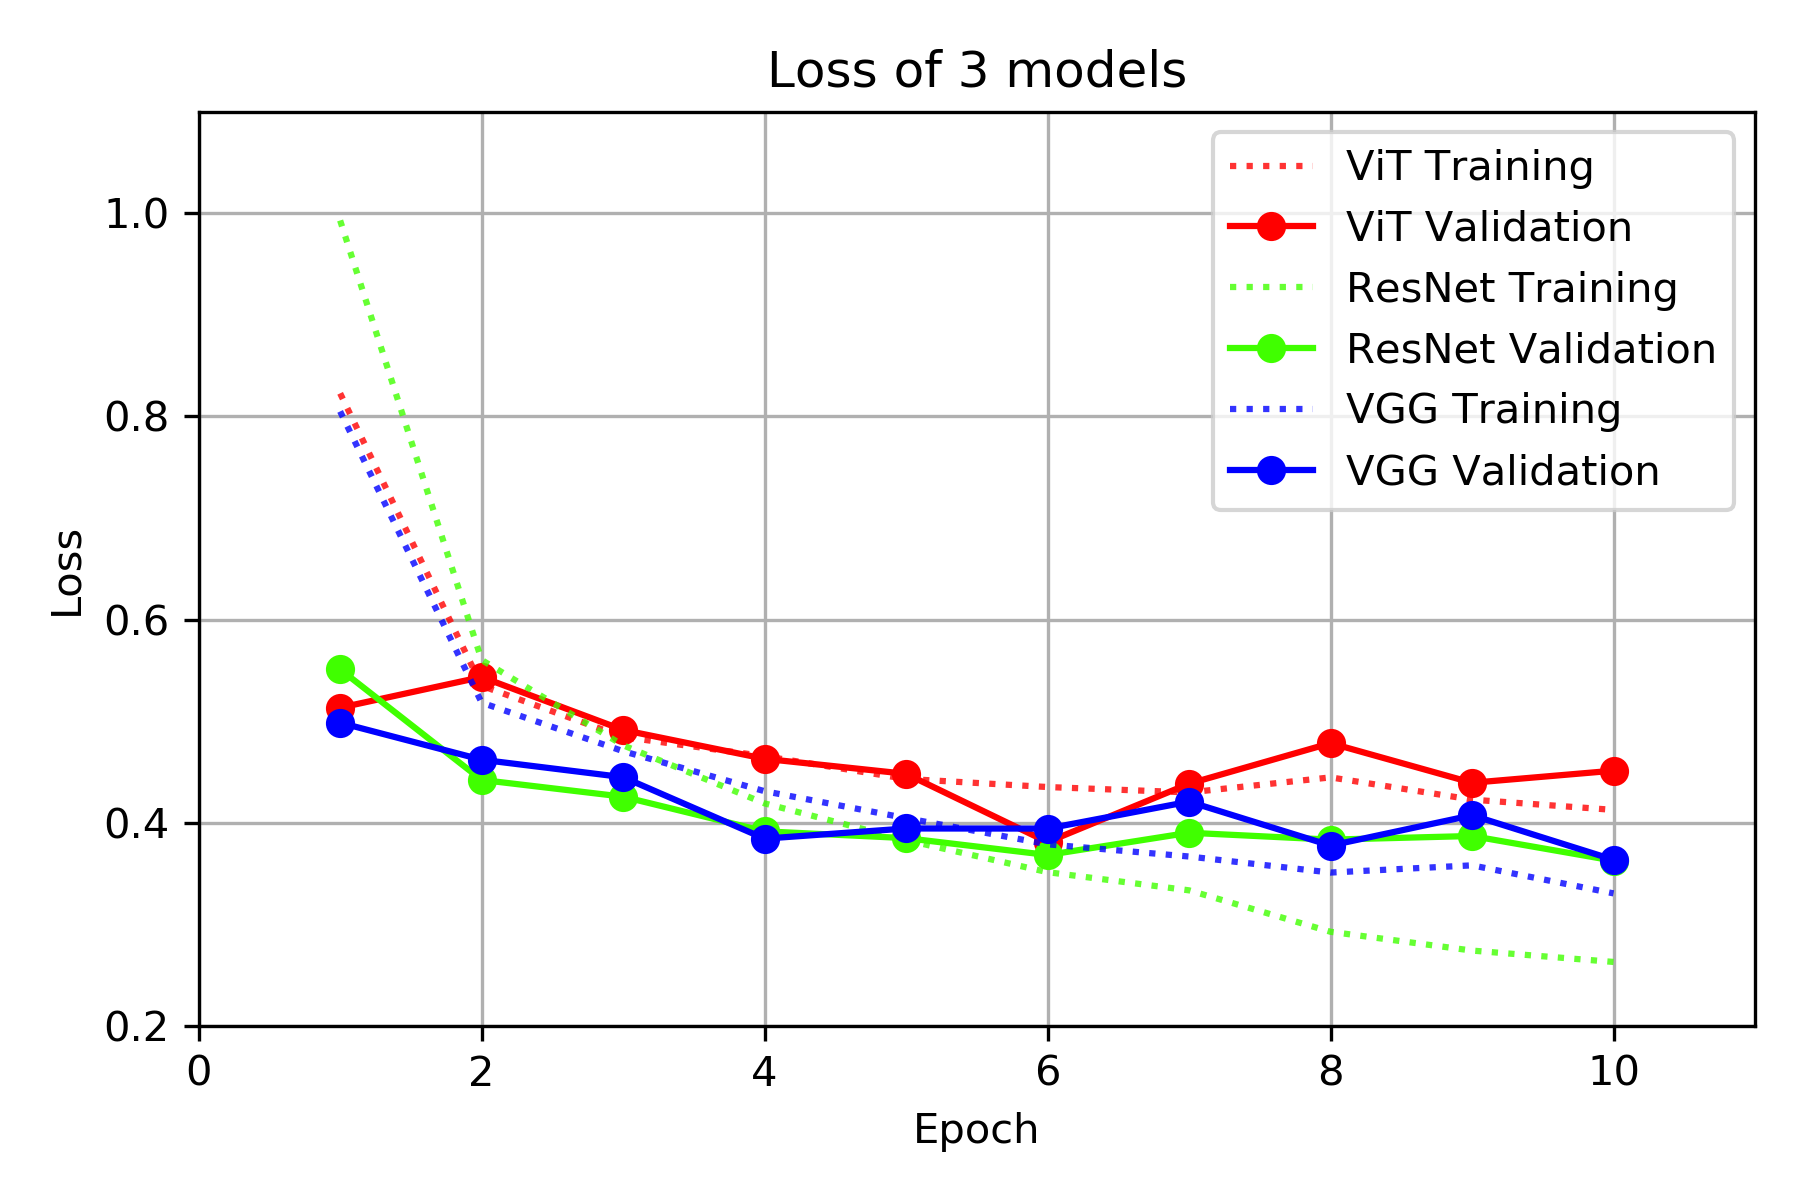
\includegraphics[keepaspectratio, scale=0.43]{figs/result3-3.png}
      \subcaption{Loss}
      %\label{fill}
    \end{minipage}
  \end{tabular}
  \caption{条件3の実験結果}
  \label{fig:re3}
\end{figure}

\newpage
\begin{table}[htbp]
  \caption{条件4の実験結果}
  \label{tb:result4}
  \centering\begin{tabular}{c|ccc}\hline
    \backslashbox{指標}{モデル} & \multicolumn{2}{c}{vit\_base\_patch\_224}\\\hline
    データセット & ILSVRC-2012 ImageNet & ImageNet-21k \\\hline
    best valid accuracy & 0.8997 & 0.9057\\\hline
    best valid f1-Score & 0.7284 & 0.7413\\\hline
    best valid loss & 0.3301 & 0.3086\\\hline
  \end{tabular}
\end{table}

%Attentionの算出過程を\fref{fig:a}に示す.
%\begin{figure}[h]
%  \centering
%  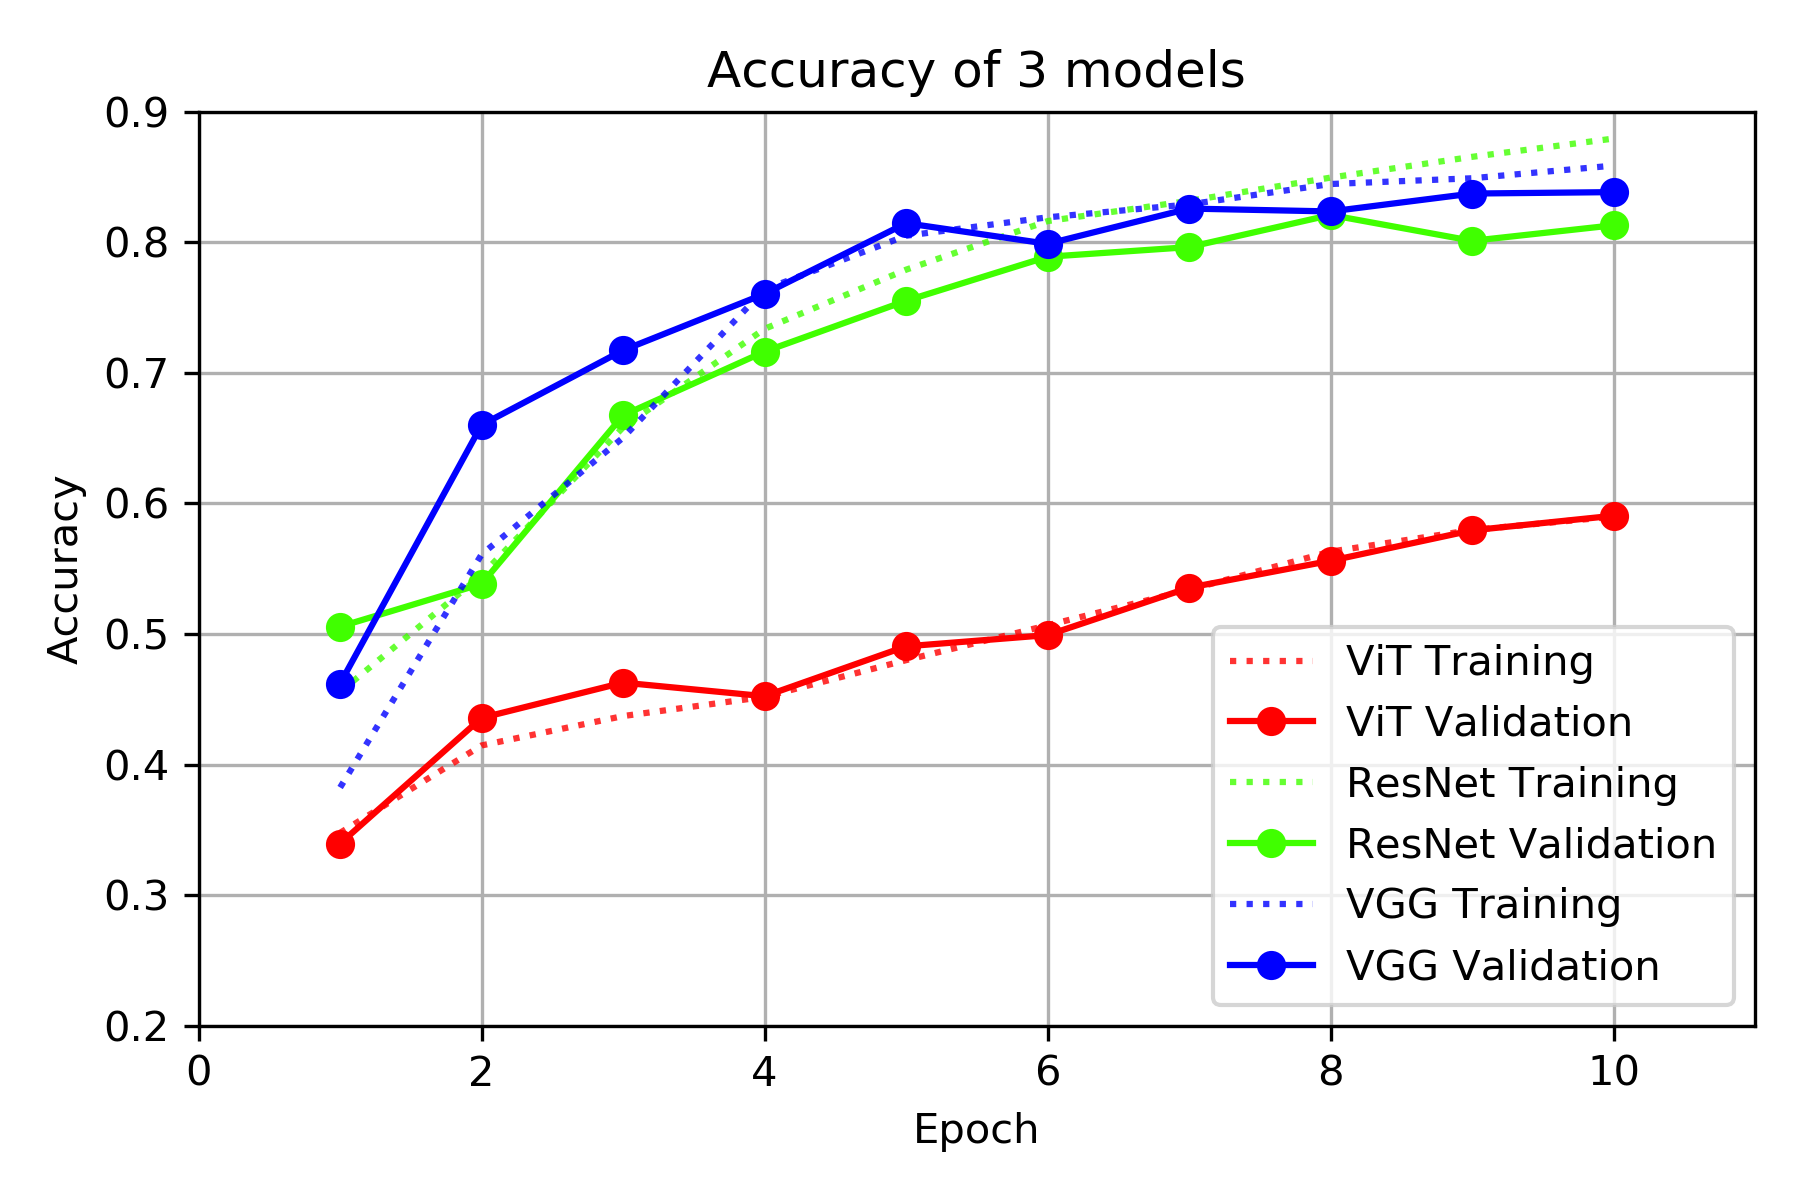
\includegraphics[width=0.9\linewidth]{figs/result1-1.png}
%  \caption{Attentionの算出過程}
%  \label{fig:a}
%\end{figure}
%条件4の各指標の結果を\fref{fig:re4}に示す.
\begin{figure}[H]
  \begin{tabular}{cc}
    \begin{minipage}[t]{0.45\hsize}
      \centering
      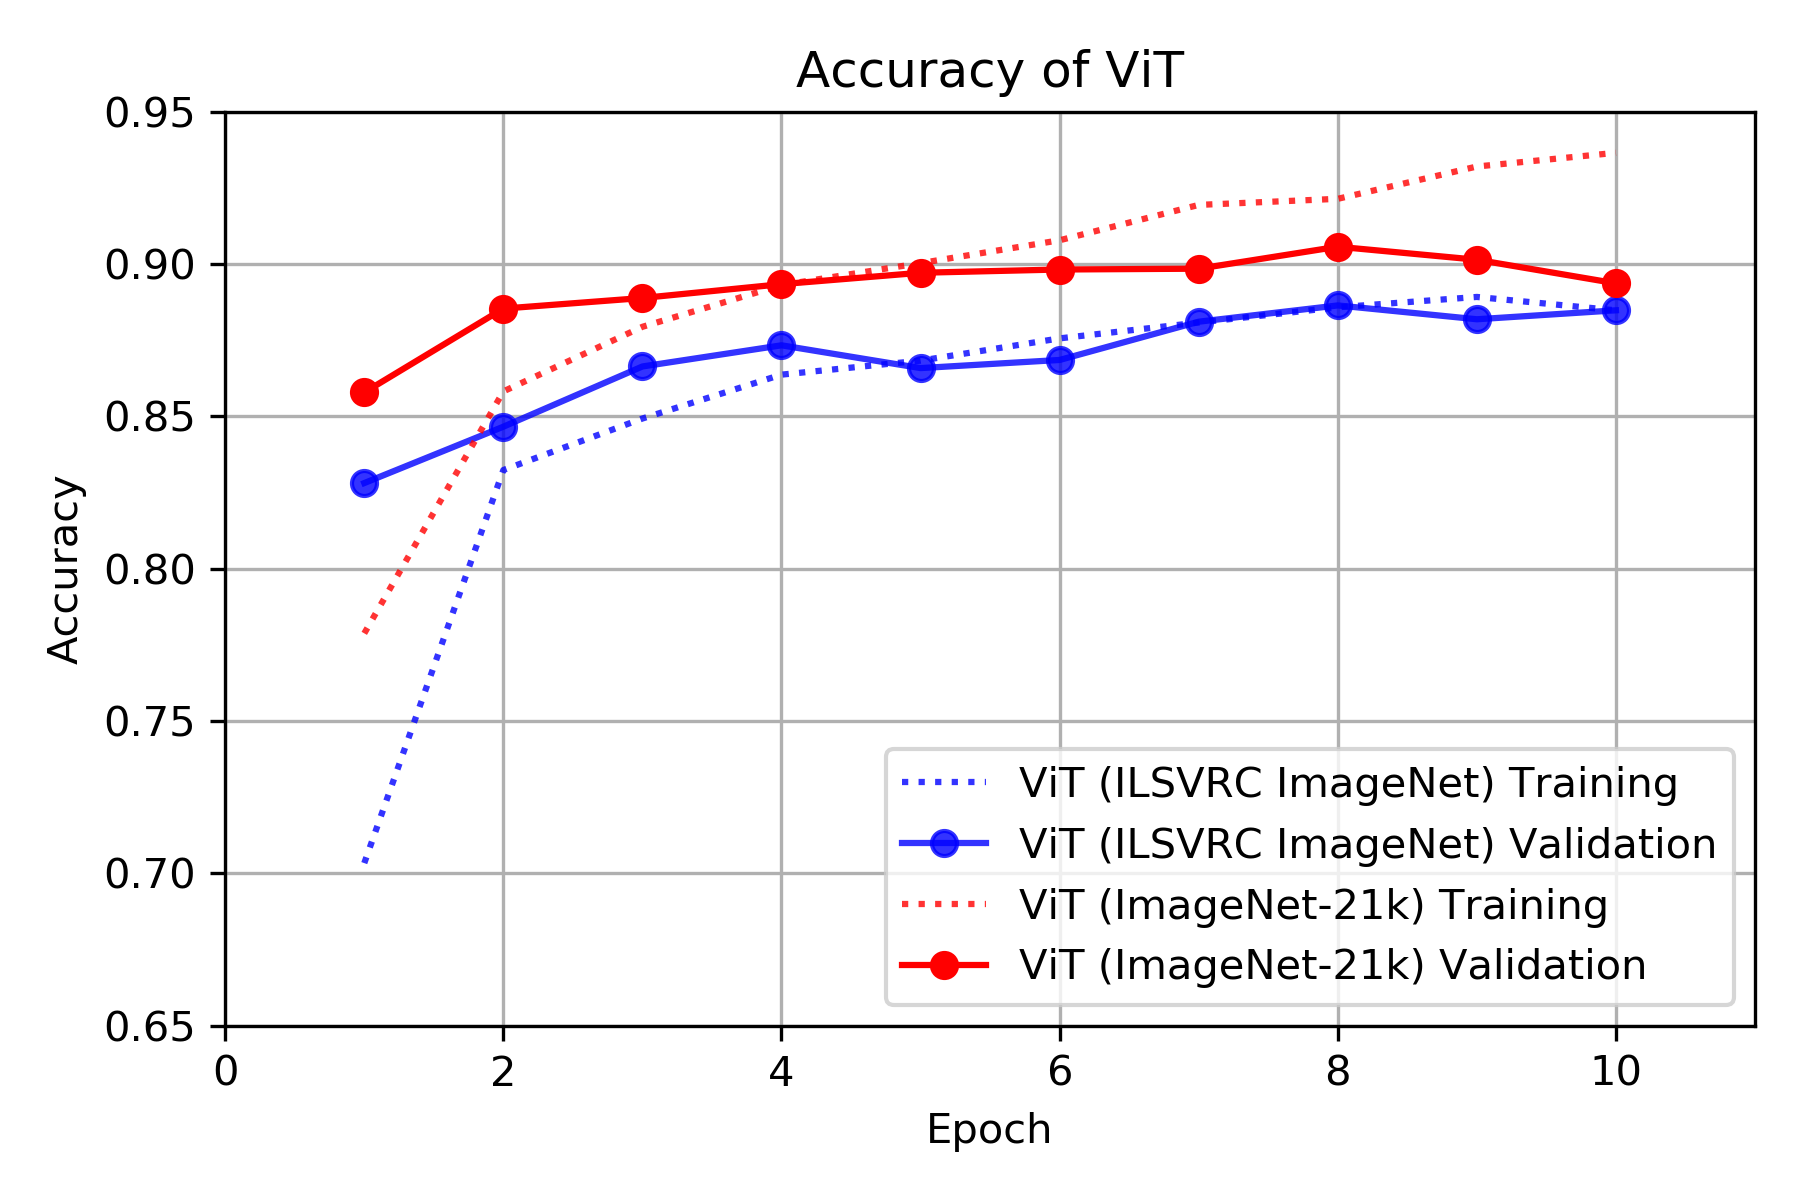
\includegraphics[keepaspectratio, scale=0.43]{figs/result4-1.png}
      \subcaption{Accuracy}
      %\label{composite}
    \end{minipage} &
    \begin{minipage}[t]{0.45\hsize}
      \centering
      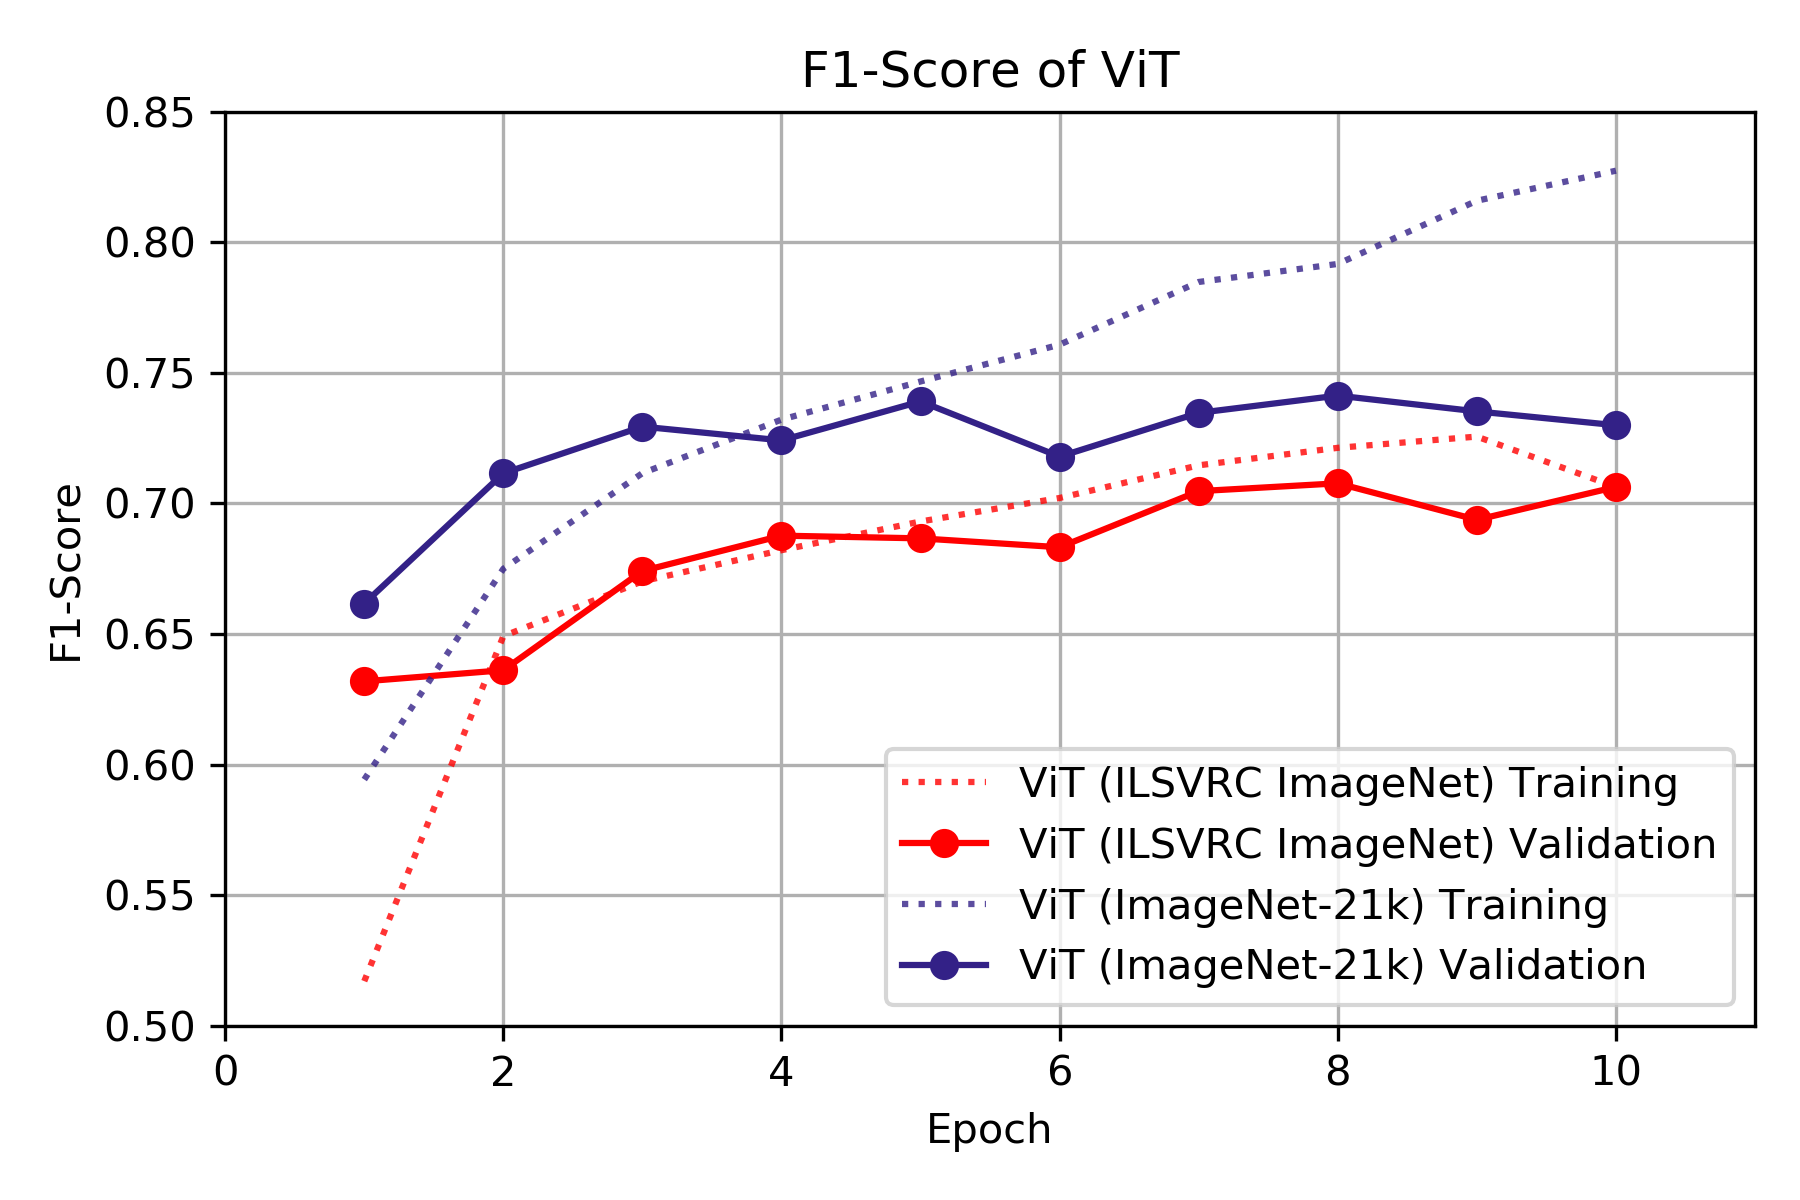
\includegraphics[keepaspectratio, scale=0.43]{figs/result4-2.png}
      \subcaption{F1-Score}
      %\label{Gradation}
    \end{minipage} \\

    \begin{minipage}[t]{0.45\hsize}
      \centering
      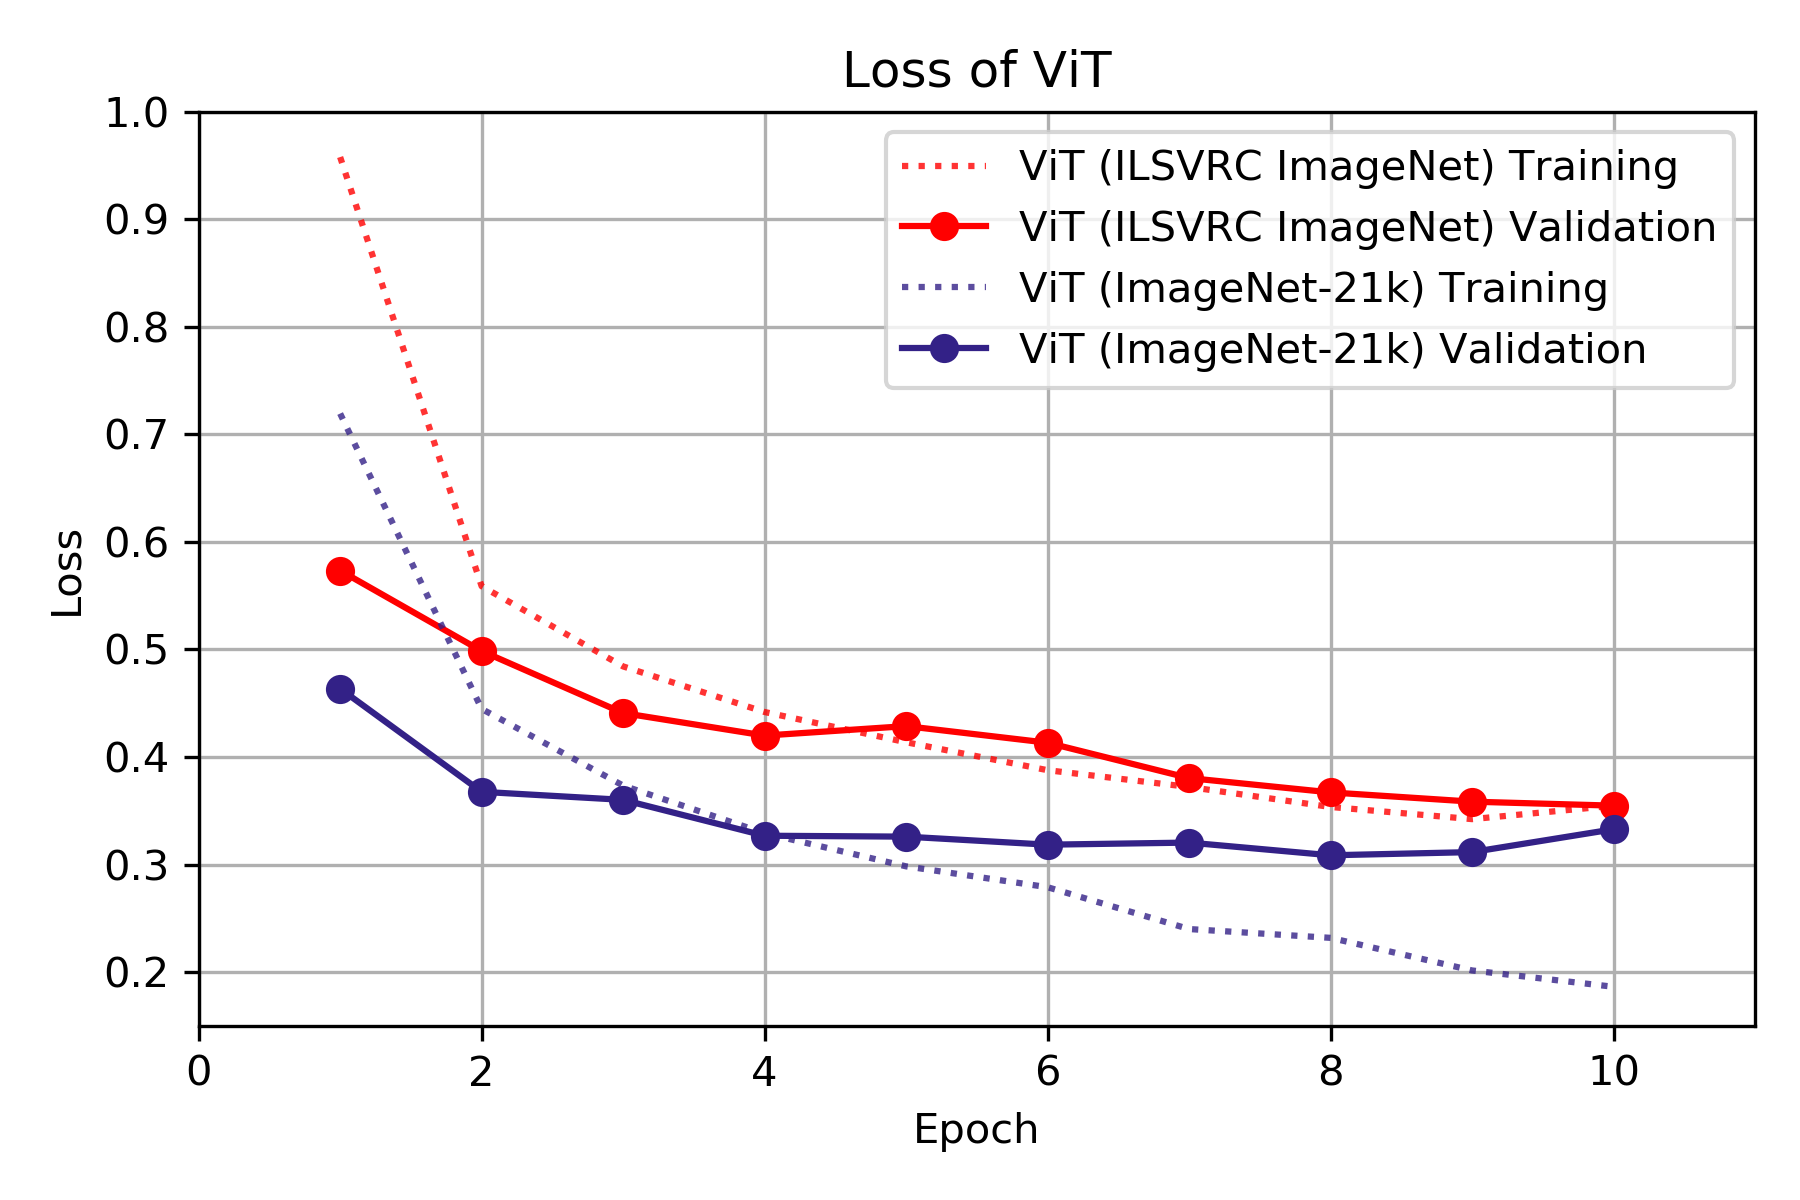
\includegraphics[keepaspectratio, scale=0.43]{figs/result4-3.png}
      \subcaption{Loss}
      %\label{fill}
    \end{minipage}
  \end{tabular}
  \caption{条件4の実験結果}
  \label{fig:re4}
\end{figure}

\chapter{議論}
条件1の実験結果より,ViTは事前学習なしの場合では良い認識結果は得られていないことがわかる.
各指標はそれぞれ良い方向に向かっているものの,ResNet,VGGには遥かに及んでいない.これは,ViTがCNNとは違い,画像に対する帰納バイアスがないことが原因だと考えられる.
帰納バイアスとは,モデルが学習する時にもっている何らかの仮定のことである.例えばCNNであれば,「畳み込み演算のように同一カーネルによる局所的な情報処理を画像全体に渡って繰り返す2次元構造」が,
帰納バイアスとして働いていて,画像認識タスクにおいて優れた性能を発揮するに至っている.このバイアスがないことが,大規模なデータセットでの事前学習がViTに対して有効で,画像認識で良い結果を出す理由の一つである.\\
%カーネルは画像全体に同じものを適用するため,CNNは移動させたカーネルと画像のスカラ積による局所性と,画像全体に渡る同一カーネルの重みの使用による移動不変性を持つ.
%移動不変性:局所的なパターンが画像内の物体位置にかかわらず、出力に対して効果的であること.局所性:近傍における局所的な演算処理

条件2の実験結果からは,事前学習をおこなった場合のViTは他2モデルより,劣っていることがわかる.また,3モデルともAccuracy・F1-Scoreはtrainingの値のみが上がり続け,Lossは限りなく0に近づいている.
そして,validationの値は横ばいになっていることがわかる.これは,モデルが訓練データに対してオーバーフィッティングし,検証データに対する予測が上手くいっていないことが原因である.
このことから次の検証では,検証データに対して汎化性能を上げるために,入力画像を加工するデータ拡張を行った.\\

条件3の実験結果では,データ拡張をおこなった場合のモデルの各指標は,training・validation共に近い値をとっており,条件2のオーバーフィッティングを解消できている.
その上,各指標の値もそれぞれ向上しており,特にViTは大きく伸びている.\\

最後にViTのみで実験を行った条件4での結果を確認する.これまでの条件と違う点は,事前学習に用いたデータセットの規模で,今までのクラス1,000,画像枚数130万枚のILSVRC-2012 ImageNetに加え,
クラス21,000,画像枚数1,400万枚のImageNet-21kを使用した点である.\fref{fig:re4}からわかるように,ViTは大規模なデータセットで学習した場合に良い認識結果を示している.
これは画像に対する帰納バイアスを持たないViTに,大量の画像による事前学習を適用したことで,ハンデを克服したと言えるだろう.しかし,ImageNet-21kで事前学習したViTは5Epochを超えたあたりから,validationとの差が広がり,オーバーフィッティングしていることもわかる.
原因は,大規模なデータセットにる事前学習の重みを適用したものの,本タスクの識別器としてはそれほど上手く機能していないことであろう.そして,この問題を解決するためには,より適切なデータ拡張やパラメータチューニングが必要だと考えられる.
また,全ての実験の結果から,今回のタスクである「リンゴの葉の病気の診断」は,画像の大域的な構造よりも診断の対照である葉の局所的なテクスチャが特徴として使われることから,CNNが得意とするタスクであり,ViT向きではなかったこともCNNとあまり差が出なかった原因の一つだとわかった.

\chapter{結論}
今回の実験で,Vision Transformerに事前学習を適用した時,
自分で選択したデータセットに対して良い認識結果が得られ,事前学習時のデータセットの規模が認識結果に関係していることもわかった.
また,データ拡張はモデルの過学習を防ぐのに貢献していた.従来のモデルとスコアがあまり変わらないのは,事前学習の画像枚数が論文の 1/230,1/20 であったことと,局所的なテクスチャが認識に重要な要素であり,ViT向きのタスクではなかったからだと考えられる.
そして,最近の研究では,畳み込み層とAttention層を組み合わせたモデルが,事前学習のデータセットの大小に関わらず,良い認識結果をもたらすこともわかっている\cite{dai2021coatnet}.
このことから,一般的に利用できる規模のデータセットで高い認識精度を得るには,画像認識に特化した局所性を持つ機構である畳み込み層と,
画像全体を参照しながら学習していくAttention層を適切に組み合わせる必要があると考えられる.

\backmatter% ここから後付
\chapter{謝辞}%%%%%%%%%%%%%%% 謝辞 %%%%%%%
本研究を進めるにあたり,ご指導くださった山口裕助教に感謝の意を表します.

% \begin{thebibliography}{}%%%% 参考文献 %%%
%   \bibitem{}
% \end{thebibliography}
\bibliographystyle{junsrt}%           BibTeX を使う場合
\bibliography{bibitem}% BibTeX を使う場合

%\appendix% ここから付録 %%%%% 付録 %%%%%%%
%\chapter{実験結果の図}
%付録があればここに書く.

\end{document}
